\chapter{Lập kế hoạch và Baseline (Task 2)}
\label{chap:task2}

% Kiểu nút dùng chung cho các sơ đồ PBS, PFD và mạng hoạt động trong chương này.
\tikzset{
  act/.style={draw, rounded corners, align=center, font=\scriptsize, text width=2.6cm, inner sep=3pt, minimum height=1cm},
  crit/.style={act, fill=red!12, draw=red!70!black, thick},
  ghost/.style={act, dashed, fill=gray!10}
}

\section{Cấu trúc phân rã sản phẩm (PBS)}
\label{sec:2-1}
PBS (Hình~\ref{fig:pbs}) chia sản phẩm của dự án thành hai nhánh: sản phẩm quản lý (M) phục vụ việc điều hành và nộp bài, và sản phẩm kỹ thuật (S) là những gì được xây dựng và bàn giao. Mỗi nút có mã để truy vết sang activity ở mục~\ref{sec:2-4}. Các module phần mềm (S31--S36) bám theo chuỗi cốt lõi mà client ưu tiên: quản lý sự kiện, đăng ký và danh sách chờ, điểm danh, báo cáo (Q08).

\begin{figure}[H]
\centering
\resizebox{\linewidth}{!}{%
\hyphenpenalty=10000 \exhyphenpenalty=10000\relax
\begin{tikzpicture}[>={Stealth[length=2mm]}]
  \node[act,text width=4.4cm] (M1) at (8.4,0.00) {\textbf{M1} Project Definition};
  \node[act,text width=4.4cm] (M2) at (8.4,-1.20) {\textbf{M2} Project Baseline};
  \node[act,text width=4.4cm] (M3) at (8.4,-2.40) {\textbf{M3} Monitoring \& Change Records};
  \node[act,text width=4.4cm] (M4) at (8.4,-3.60) {\textbf{M4} Final Report \& Closure};
  \node[act,text width=3.6cm] (M) at (3.6,-1.80) {\textbf{M} Management Products};
  \node[act,text width=4.4cm] (S1) at (8.4,-4.80) {\textbf{S1} Validated Scope \& Requirements};
  \node[act,text width=5.8cm] (S21) at (15.2,-6.00) {\textbf{S21} Database Design};
  \node[act,text width=5.8cm] (S22) at (15.2,-7.20) {\textbf{S22} API Contract};
  \node[act,text width=4.4cm] (S2) at (8.4,-6.60) {\textbf{S2} System Design};
  \node[act,text width=5.8cm] (S31) at (15.2,-8.40) {\textbf{S31} Authentication \& Authorization};
  \node[act,text width=5.8cm] (S32) at (15.2,-9.60) {\textbf{S32} Event Management};
  \node[act,text width=5.8cm] (S33) at (15.2,-10.80) {\textbf{S33} Registration \& Waitlist};
  \node[act,text width=5.8cm] (S34) at (15.2,-12.00) {\textbf{S34} Check-in \& Attendance};
  \node[act,text width=5.8cm] (S35) at (15.2,-13.20) {\textbf{S35} Reporting \& Export};
  \node[act,text width=5.8cm] (S36) at (15.2,-14.40) {\textbf{S36} User Interface};
  \node[act,text width=4.4cm] (S3) at (8.4,-11.40) {\textbf{S3} Software Products};
  \node[act,text width=5.8cm] (S41) at (15.2,-15.60) {\textbf{S41} Test Specification};
  \node[act,text width=5.8cm] (S42) at (15.2,-16.80) {\textbf{S42} Tested Integrated System};
  \node[act,text width=4.4cm] (S4) at (8.4,-16.20) {\textbf{S4} Test Products};
  \node[act,text width=5.8cm] (S51) at (15.2,-18.00) {\textbf{S51} Deployed System};
  \node[act,text width=5.8cm] (S52) at (15.2,-19.20) {\textbf{S52} Handover Documentation};
  \node[act,text width=4.4cm] (S5) at (8.4,-18.60) {\textbf{S5} Release Products};
  \node[act,text width=3.6cm] (S) at (3.6,-11.70) {\textbf{S} Specialist Products};
  \node[act,text width=3.4cm] (P0) at (-1.6,-6.75) {\textbf{P0} University Event Registration System};
  \draw[->] (M.east) to[out=0,in=180] (M1.west);
  \draw[->] (M.east) to[out=0,in=180] (M2.west);
  \draw[->] (M.east) to[out=0,in=180] (M3.west);
  \draw[->] (M.east) to[out=0,in=180] (M4.west);
  \draw[->] (S.east) to[out=0,in=180] (S1.west);
  \draw[->] (S2.east) to[out=0,in=180] (S21.west);
  \draw[->] (S2.east) to[out=0,in=180] (S22.west);
  \draw[->] (S.east) to[out=0,in=180] (S2.west);
  \draw[->] (S3.east) to[out=0,in=180] (S31.west);
  \draw[->] (S3.east) to[out=0,in=180] (S32.west);
  \draw[->] (S3.east) to[out=0,in=180] (S33.west);
  \draw[->] (S3.east) to[out=0,in=180] (S34.west);
  \draw[->] (S3.east) to[out=0,in=180] (S35.west);
  \draw[->] (S3.east) to[out=0,in=180] (S36.west);
  \draw[->] (S.east) to[out=0,in=180] (S3.west);
  \draw[->] (S4.east) to[out=0,in=180] (S41.west);
  \draw[->] (S4.east) to[out=0,in=180] (S42.west);
  \draw[->] (S.east) to[out=0,in=180] (S4.west);
  \draw[->] (S5.east) to[out=0,in=180] (S51.west);
  \draw[->] (S5.east) to[out=0,in=180] (S52.west);
  \draw[->] (S.east) to[out=0,in=180] (S5.west);
  \draw[->] (P0.east) to[out=0,in=180] (M.west);
  \draw[->] (P0.east) to[out=0,in=180] (S.west);
\end{tikzpicture}}
\caption{Cấu trúc phân rã sản phẩm (PBS)}
\label{fig:pbs}
\end{figure}

Sơ đồ là kết quả A15 (TV3, TV5); bộ mã M/S là mã sản phẩm chính thức của dự án (TV1 chốt 20/10).

\section{Mô tả sản phẩm (Product Descriptions)}
\label{sec:2-2}
Năm Product Description dưới đây mô tả các sản phẩm quyết định việc nghiệm thu và kiểm thử: S1, S21, S34, S41, S51 (mã theo PBS ở mục~\ref{sec:2-1}). Mỗi PD gồm các trường định danh, mục đích, nguồn tạo ra, thành phần, định dạng, tiêu chuẩn liên quan, tiêu chí chất lượng và phương pháp kiểm tra. Nội dung lấy từ tab Product Description của Sheet master; các PD được thành viên duyệt ngày 14/10, bổ sung ngày 20/10 theo phản hồi Q12, Q19, Q20 và stack đã chốt (React, Go, PostgreSQL).

\subsection*{PD-01 -- S1 Validated Scope \& Requirements}
\noindent\textit{TV2 duyệt 14/10; bổ sung Q12, Q19, Q20 ngày 20/10.}

\begingroup\tblsetup\tblzebra
\begin{longtable}{L{3.4cm}L{11.6cm}}
\caption{PD-01 -- S1 Validated Scope \& Requirements}\label{tab:pd-01}\\
\toprule
\rowcolor{tblheadbg}\textbf{Trường} & \textbf{Nội dung} \\
\midrule
\endfirsthead
\toprule
\rowcolor{tblheadbg}\textbf{Trường} & \textbf{Nội dung} \\
\midrule
\endhead
\bottomrule
\endlastfoot
Định danh & S1 Đặc tả yêu cầu (Validated Scope \& Requirements) \\
Mục đích & Mô tả đầy đủ yêu cầu chức năng và phi chức năng đã được client xác nhận, làm đầu vào cho thiết kế, kiểm thử và Baseline V1.0 \\
Nguồn tạo ra (derivation) & Client Interaction Log (Q01–Q20), scope và MoE (A07), giả định ASM-01 đến ASM-07 \\
Thành phần & Danh sách REQ-01 đến REQ-21 có mức MoSCoW và tiêu chí chấp nhận; ràng buộc phi chức năng; giả định và loại trừ; quy tắc nghiệp vụ đã xác nhận (hạn hủy 24 giờ, waitlist FIFO, một đăng ký còn hiệu lực/sinh viên/sự kiện; Organizer không tự duyệt sự kiện mình tạo, Admin duyệt (Q12); Organizer sửa/hủy sự kiện sau công bố, đổi thời gian/địa điểm phải thông báo (Q19); quyền xem dữ liệu theo vai trò và đơn vị (Q20)) \\
Định dạng & Markdown trong \texttt{docs/task2}, xuất sang báo cáo mục 1.4 \\
Tiêu chuẩn liên quan & Mỗi requirement có mã duy nhất và truy ngược được về câu trả lời của client hoặc assumption có mã \\
Tiêu chí chất lượng & 100\% requirement Must có tiêu chí chấp nhận kiểm tra được; 100\% truy ngược được về Client Log hoặc assumption; không có mâu thuẫn giữa bảng MoSCoW và báo cáo \\
Phương pháp và người kiểm tra & Review chéo bởi TV1 theo checklist CP2; client đã xác nhận scope ở Q10 và Q11 \\
\end{longtable}
\endgroup

\subsection*{PD-02 -- S21 Database Design}
\noindent\textit{TV4, TV3 duyệt 14/10; bổ sung bảng units, notifications và stack ngày 20/10, chờ TV3 xác nhận.}

\begingroup\tblsetup\tblzebra
\begin{longtable}{L{3.4cm}L{11.6cm}}
\caption{PD-02 -- S21 Database Design}\label{tab:pd-02}\\
\toprule
\rowcolor{tblheadbg}\textbf{Trường} & \textbf{Nội dung} \\
\midrule
\endfirsthead
\toprule
\rowcolor{tblheadbg}\textbf{Trường} & \textbf{Nội dung} \\
\midrule
\endhead
\bottomrule
\endlastfoot
Định danh & S21 Thiết kế cơ sở dữ liệu (ERD và schema) \\
Mục đích & Mô hình dữ liệu đáp ứng mọi requirement Must và các quy tắc nghiệp vụ đã xác nhận \\
Nguồn tạo ra (derivation) & S1 Validated Scope \& Requirements; ASM-02 (quy mô) \\
Thành phần & ERD; định nghĩa bảng users, roles, units (đơn vị tổ chức, Q01, Q20), events, registrations, waitlist, attendance, notifications (thông báo trong ứng dụng, Q14, Q19); khóa, ràng buộc, chỉ mục; trạng thái sự kiện gồm Cancelled (Q19); waitlist có thứ tự FIFO, tự chuyển đầu waitlist và tạo thông báo (Q14); đăng ký còn hiệu lực hoặc đã hủy, lưu thời điểm để đăng ký lại vào cuối waitlist (Q15) \\
Định dạng & Sơ đồ ERD; file migration SQL cho PostgreSQL trong mã nguồn backend (Go) \\
Tiêu chuẩn liên quan & Chuẩn hóa tới 3NF trừ khi có lý do ghi rõ; tên bảng và cột snake\_case \\
Tiêu chí chất lượng & Mọi requirement Must ánh xạ được vào thực thể; ràng buộc không đăng ký trùng và không vượt số chỗ được thực thi ở mức database; tự chuyển đầu waitlist đúng một lần, không chuyển trùng; thông báo lỗi vẫn giữ đăng ký chính thức; test đồng thời 100 lượt đăng ký không vượt chỗ \\
Phương pháp và người kiểm tra & Review bởi TV3 và TV4 (frontend dùng được); test FIFO và đồng thời, test tích hợp với dữ liệu mẫu 500 lượt đăng ký \\
\end{longtable}
\endgroup

\subsection*{PD-03 -- S34 Check-in \& Attendance}
\noindent\textit{TV4 duyệt 14/10; bổ sung stack và quyền điểm danh 20/10.}

\begingroup\tblsetup\tblzebra
\begin{longtable}{L{3.4cm}L{11.6cm}}
\caption{PD-03 -- S34 Check-in \& Attendance}\label{tab:pd-03}\\
\toprule
\rowcolor{tblheadbg}\textbf{Trường} & \textbf{Nội dung} \\
\midrule
\endfirsthead
\toprule
\rowcolor{tblheadbg}\textbf{Trường} & \textbf{Nội dung} \\
\midrule
\endhead
\bottomrule
\endlastfoot
Định danh & S34 Module điểm danh (Check-in \& Attendance) \\
Mục đích & Ghi nhận người tham dự nhanh và chính xác tại sự kiện, kể cả khi QR không dùng được \\
Nguồn tạo ra (derivation) & S33 Registration \& Waitlist; kết quả spike A20; Q03 \\
Thành phần & Sinh mã QR cho đăng ký; màn hình quét; nhập mã hoặc xác nhận thủ công; chặn điểm danh trùng; lưu thời điểm; không check-out \\
Định dạng & Mã nguồn giao diện quét (React) và API điểm danh (Go), chạy trên bản deploy \\
Tiêu chuẩn liên quan & Hoạt động trên trình duyệt điện thoại, mobile-first, không cần cài ứng dụng \\
Tiêu chí chất lượng & Median thời gian điểm danh $\le$ 5 giây trong môi trường test của nhóm (O2); không tạo bản ghi điểm danh trùng; phương án thủ công cập nhật giống QR; chỉ Organizer của sự kiện hoặc Admin được điểm danh (Q20) \\
Phương pháp và người kiểm tra & Test trên ít nhất 3 thiết bị thật; test case T-CI-01 đến T-CI-05 (đề xuất, mã chốt ở A22); review bởi TV2 \\
\end{longtable}
\endgroup

\subsection*{PD-04 -- S41 Test Specification}
\noindent\textit{TV2 duyệt 14/10.}

\begingroup\tblsetup\tblzebra
\begin{longtable}{L{3.4cm}L{11.6cm}}
\caption{PD-04 -- S41 Test Specification}\label{tab:pd-04}\\
\toprule
\rowcolor{tblheadbg}\textbf{Trường} & \textbf{Nội dung} \\
\midrule
\endfirsthead
\toprule
\rowcolor{tblheadbg}\textbf{Trường} & \textbf{Nội dung} \\
\midrule
\endhead
\bottomrule
\endlastfoot
Định danh & S41 Đặc tả kiểm thử (test plan và test case) \\
Mục đích & Mô tả kế hoạch và test case để kiểm tra các requirement; là bằng chứng cho Task 3.5 và đầu vào cho UAT. Kết quả chạy test được lưu riêng. \\
Nguồn tạo ra (derivation) & S1 Validated Scope \& Requirements; quality plan (A22) \\
Thành phần & Chiến lược test theo mức (unit, integration, e2e, UAT); test case có mã gắn với requirement; dữ liệu test; tiêu chí pass/fail; nơi lưu kết quả \\
Định dạng & Markdown trong \texttt{docs/quality} và test tự động trong \texttt{src/} \\
Tiêu chuẩn liên quan & Mã test theo quy ước T-nhóm-số (ví dụ T-REG-01), gắn với REQ \\
Tiêu chí chất lượng & 100\% requirement Must có ít nhất một test case; mỗi test case có kết quả kỳ vọng đo được; 100\% test đã chạy được ghi kết quả \\
Phương pháp và người kiểm tra & Review bởi TV1 và TV4; kết quả chạy lưu và liên kết từ ma trận truy vết \\
\end{longtable}
\endgroup

\subsection*{PD-05 -- S51 Deployed System}
\noindent\textit{TV2 duyệt 14/10.}

\begingroup\tblsetup\tblzebra
\begin{longtable}{L{3.4cm}L{11.6cm}}
\caption{PD-05 -- S51 Deployed System}\label{tab:pd-05}\\
\toprule
\rowcolor{tblheadbg}\textbf{Trường} & \textbf{Nội dung} \\
\midrule
\endfirsthead
\toprule
\rowcolor{tblheadbg}\textbf{Trường} & \textbf{Nội dung} \\
\midrule
\endhead
\bottomrule
\endlastfoot
Định danh & S51 Hệ thống đã triển khai \\
Mục đích & Sản phẩm chạy được để client nghiệm thu và nhóm demo \\
Nguồn tạo ra (derivation) & S42 Tested Integrated System (toàn bộ module S31 đến S36) \\
Thành phần & Ứng dụng đang chạy; database có dữ liệu mẫu (500 lượt đăng ký); 3 tài khoản demo cho Student, Organizer, Admin (ASM-06); README hướng dẫn chạy \\
Định dạng & URL bản deploy và mã nguồn trong repo (bản mirror công khai) \\
Tiêu chuẩn liên quan & Chạy trên trình duyệt phổ biến và điện thoại; không lưu mật khẩu hay dữ liệu thật trong repo \\
Tiêu chí chất lượng & Luồng tạo sự kiện, duyệt, đăng ký, waitlist, check-in, báo cáo chạy không lỗi nghiêm trọng; người ngoài nhóm dựng lại được theo README trong dưới 30 phút \\
Phương pháp và người kiểm tra & Regression test A39; UAT A41; review bởi TV5 \\
\end{longtable}
\endgroup

\kiemtra{PD-02: phần bổ sung ngày 20/10 (bảng units, notifications; migration PostgreSQL) chờ TV3 xác nhận. PD-03: mã test T-CI-01 đến T-CI-05 là đề xuất, mã chính thức chốt ở A22.}

\section{Sơ đồ luồng sản phẩm (PFD)}
\label{sec:2-3}
PFD (Hình~\ref{fig:pfd}) cho biết sản phẩm nào là đầu vào để tạo ra sản phẩm nào. Đây là quan hệ dẫn xuất giữa sản phẩm, không phải thứ tự công việc; thứ tự công việc nằm ở mạng hoạt động (mục~\ref{sec:2-4}).

\begin{figure}[H]
\centering
\resizebox{0.95\linewidth}{!}{%
\hyphenpenalty=10000 \exhyphenpenalty=10000\relax
\begin{tikzpicture}[>={Stealth[length=2mm]}]
  \node[act,text width=3.4cm] (REQ) at (6.00,0.00) {Validated Scope \& Requirements};
  \node[act,text width=3.4cm] (DB) at (0.00,-1.90) {Database Design};
  \node[act,text width=3.4cm] (API) at (4.00,-1.90) {API Contract};
  \node[act,text width=3.4cm] (TEST) at (8.00,-1.90) {Test Specification};
  \node[act,text width=3.4cm] (UI) at (12.00,-1.90) {User Interface};
  \node[act,text width=3.4cm] (AUTH) at (8.00,-3.80) {Authentication \& Authorization};
  \node[act,text width=3.4cm] (EVENT) at (2.40,-3.80) {Event Management};
  \node[act,text width=3.4cm] (REG) at (2.40,-5.70) {Registration \& Waitlist};
  \node[act,text width=3.4cm] (CHECK) at (2.40,-7.60) {Check-in \& Attendance};
  \node[act,text width=3.4cm] (REPORT) at (2.40,-9.50) {Reporting \& Export};
  \node[act,text width=3.4cm] (SYS) at (2.40,-11.40) {Tested Integrated System};
  \node[act,text width=3.4cm] (DEPLOY) at (2.40,-13.30) {Deployed System};
  \node[act,text width=3.4cm] (HAND) at (2.40,-15.20) {Handover Documentation};
  \draw[->] (REQ) -- (DB);
  \draw[->] (REQ) -- (API);
  \draw[->] (REQ) -- (TEST);
  \draw[->] (REQ) -- (UI);
  \draw[->] (DB) -- (EVENT);
  \draw[->] (API) -- (EVENT);
  \draw[->] (DB) -- (AUTH);
  \draw[->] (API) -- (AUTH);
  \draw[->] (EVENT) -- (REG);
  \draw[->] (REG) -- (CHECK);
  \draw[->] (CHECK) -- (REPORT);
  \draw[->] (REPORT) -- (SYS);
  \draw[->] (SYS) -- (DEPLOY);
  \draw[->] (DEPLOY) -- (HAND);
  \draw[->] (REG.west) to[out=180,in=180,looseness=1.4] (REPORT.west);
  \draw[->] (EVENT.west) to[out=180,in=180,looseness=1] (SYS.west);
  \draw[->] (REG.west) to[out=180,in=180,looseness=1.2] (SYS.west);
  \draw[->] (CHECK.west) to[out=180,in=180,looseness=1.4] (SYS.west);
  \draw[->] (AUTH.east) to[out=0,in=0,looseness=1] (SYS.east);
  \draw[->] (TEST.east) to[out=0,in=0,looseness=1] (SYS.east);
  \draw[->] (UI.east) to[out=0,in=0,looseness=1] (SYS.east);
\end{tikzpicture}}
\caption{Sơ đồ luồng sản phẩm (PFD)}
\label{fig:pfd}
\end{figure}

Sơ đồ là kết quả A15 (TV3, TV5).

\section{Mạng hoạt động}
\label{sec:2-4}
Activity được suy ra từ PFD: mỗi sản phẩm trong PFD có ít nhất một activity tạo ra nó. Tên activity theo dạng động từ cộng danh từ; quan hệ phụ thuộc là finish-to-start; các mốc theo lịch môn học (hỏi client, duyệt baseline, Progress Check, UAT, demo) được đặt ràng buộc không bắt đầu trước ngày cố định. Mạng được chia làm ba hình: lập kế hoạch đến chốt baseline (Hình~\ref{fig:net-a}), Increment 1 và Increment 2 đến Progress Check (Hình~\ref{fig:net-b}), kiểm thử Increment 2 đến demo (Hình~\ref{fig:net-c}). Mỗi nút ghi effort, thời lượng CPM, ngày theo lịch đã san tải, người làm và float CPM (mục~\ref{sec:2-11}). Nút viền đỏ là đường găng sau san tải; nút nét đứt là activity thuộc hình khác; cạnh nét đứt xanh là phụ thuộc được sửa ở L8--L11 (A21, A50).

\begin{figure}[p]
\centering
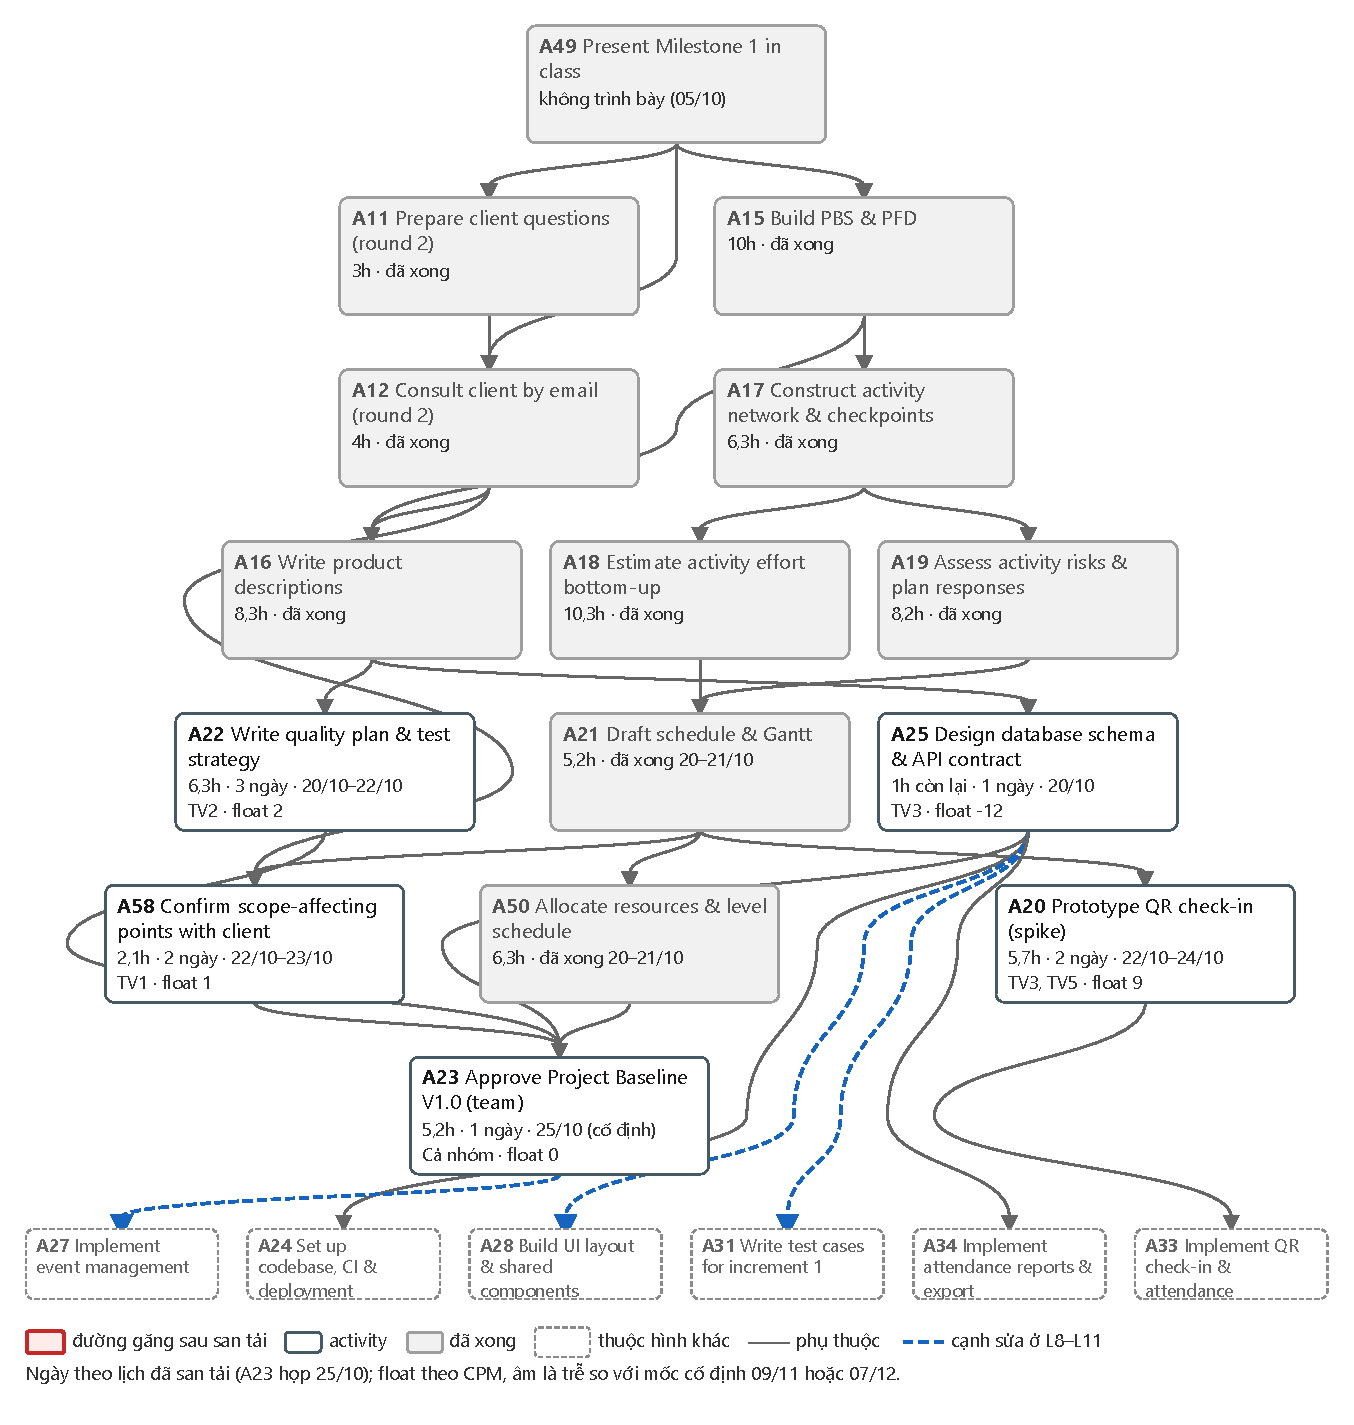
\includegraphics[width=\linewidth,height=0.9\textheight,keepaspectratio]{image/network-a.pdf}
\caption{Mạng hoạt động -- từ PBS/PFD đến chốt Baseline V1.0 (A23, 25/10)}
\label{fig:net-a}
\end{figure}

\begin{figure}[p]
\centering
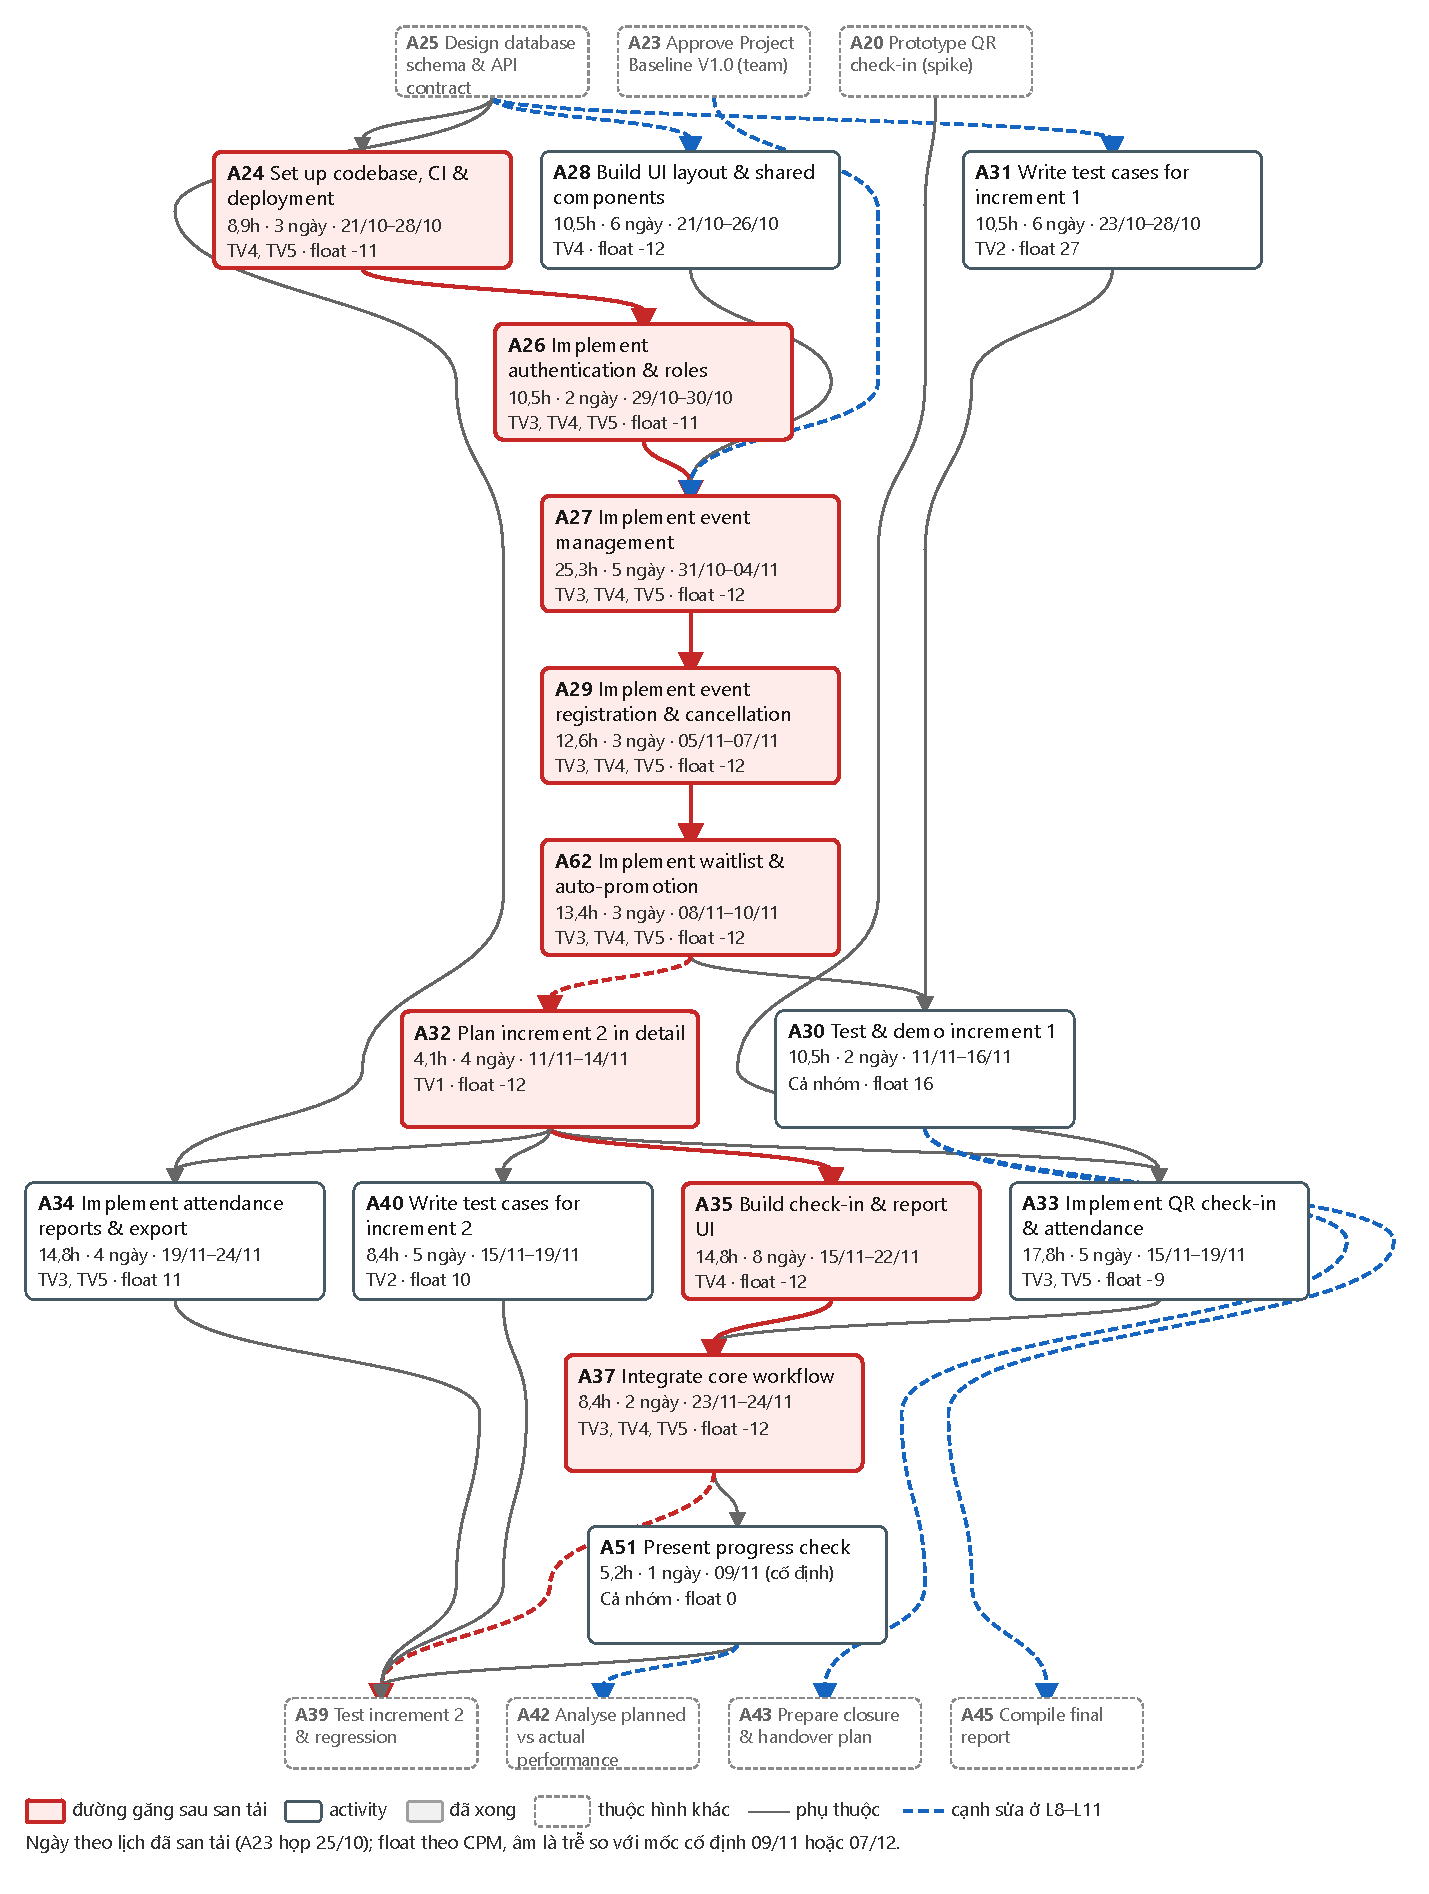
\includegraphics[width=\linewidth,height=0.9\textheight,keepaspectratio]{image/network-b.pdf}
\caption{Mạng hoạt động -- Increment 1 và Increment 2 đến Progress Check (A51, 09/11)}
\label{fig:net-b}
\end{figure}

\begin{figure}[p]
\centering
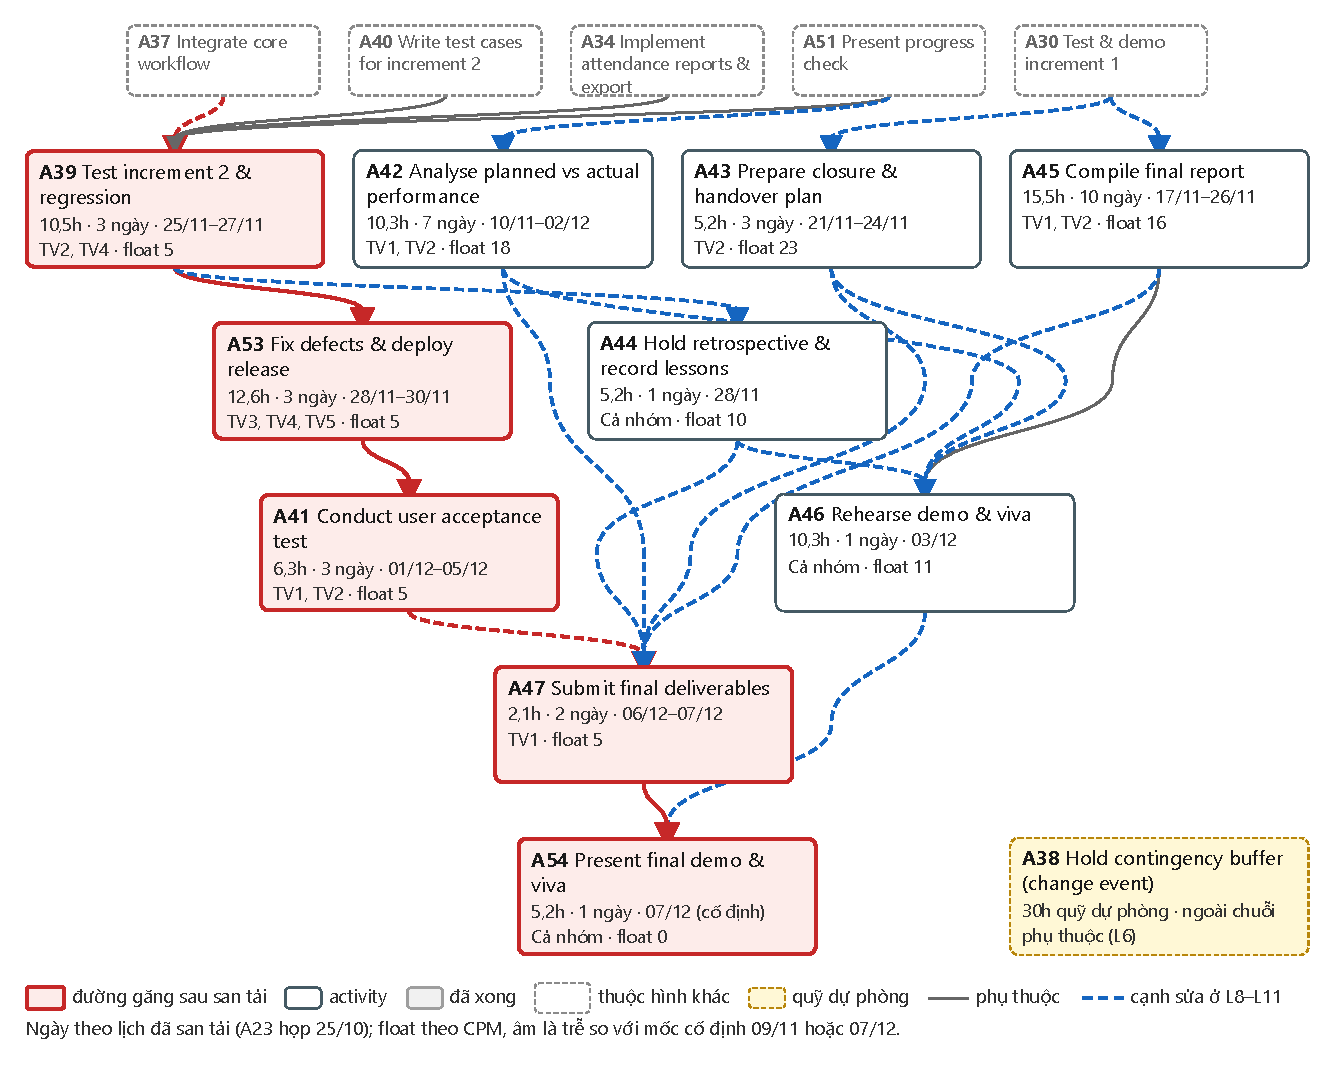
\includegraphics[width=\linewidth,height=0.9\textheight,keepaspectratio]{image/network-c.pdf}
\caption{Mạng hoạt động -- kiểm thử Increment 2, nghiệm thu, đóng dự án và demo; A38 là quỹ dự phòng ngoài chuỗi}
\label{fig:net-c}
\end{figure}

Các activity xuyên suốt A36 (giám sát tiến độ) và A57 (rà soát truy vết) là hammock chạy nền từ sau A23 đến 07/12 nên không vẽ trong sơ đồ; chúng có trên Gantt (Hình~\ref{fig:gantt}). Đường găng trong sơ đồ là kết quả CPM và san tải ở A21, A50.

Khi đối chiếu PFD với mạng hoạt động, nhóm phát hiện các điểm lệch dưới đây; PM chốt cách xử lý từ 12 đến 15/10 và nhóm duyệt tại CP2 ngày 18/10.
\begin{itemize}
  \item \textbf{Báo cáo và điểm danh:} PFD cho điểm danh đi trước báo cáo. Để không làm trễ Progress Check 09/11, A34 (báo cáo) làm gối đầu A33 (điểm danh), bắt đầu sau A32 và A25 trên dữ liệu mẫu; A37 chỉ gồm A33 và A35; báo cáo được tích hợp và kiểm với dữ liệu điểm danh thật ở A39. Đây là lệch khỏi PFD có chủ đích. PM chọn ngày 13/10 trong các phương án AI đề xuất, TV3 xác nhận khả thi ngày 14/10.
  \item \textbf{Danh sách chờ:} client xác nhận danh sách chờ với tự động chuyển người là một phần của workflow cốt lõi (Q04, Q08). Activity đăng ký cũ được tách thành A29 (đăng ký, hủy) và A62 (danh sách chờ, tự động chuyển, thông báo); quy tắc chi tiết đã được client xác nhận ở vòng 2 (Q14, Q15).
  \item \textbf{Sửa hoặc hủy sự kiện đã công bố:} yêu cầu mới từ phản hồi 08/10 (Q19), ảnh hưởng A27 (quản lý sự kiện) và A29 (hủy đăng ký theo sự kiện). Phần sửa, hủy sự kiện và thông báo được tính trong A27, không tính trùng ở A29 (TV3 xác nhận 14/10).
  \item \textbf{Triển khai bản cuối:} activity A53 được mở rộng thành sửa lỗi và triển khai bản phát hành, để sản phẩm Deployed System có activity tạo ra.
  \item \textbf{Spike QR:} A20 không còn chặn A24 (dựng codebase); A24 chờ A25 vì cần thiết kế và stack đã chốt; A20 phải xong trước A33 để kết quả spike là đầu vào của điểm danh (PM chốt 15/10).
\end{itemize}

Khi lập lịch ở A21 và san tải ở A50 (20/10), PM chọn thêm bốn thay đổi phụ thuộc trong các phương án AI đề xuất; nhóm xác nhận tại A23:
\begin{itemize}
  \item \textbf{L8 -- gối đầu Increment 1:} A24, A28, A31 bắt đầu sau A25, A26 sau A24, không chờ A23; A27 chờ A23. Lý do: CP2 đã duyệt scope, điều kiện còn lại chỉ là lịch và tài nguyên.
  \item \textbf{L9 -- chuyển việc khỏi TV1:} TV2 thực hiện khoảng 19 giờ (A22, A43, phần kiểm thử của A42, A45), TV1 vẫn là owner và người duyệt; A34 làm chung TV3, TV5; A39 làm chung TV2, TV4.
  \item \textbf{L10 -- việc đóng dự án bắt đầu sớm:} A43, A45 sau A30; A42 sau A51; A44 sau A39; A46, A47 chờ A42--A45; A54 sau A46, A47.
  \item \textbf{L11:} A32 (lập kế hoạch Increment 2) sau A62, làm song song A30, vì A32 nằm trên đường găng.
\end{itemize}

\kiemtra{Hình~\ref{fig:net-a}--\ref{fig:net-c} do AI hỗ trợ vẽ ngày 21/10 bằng script trong \texttt{tools/diagrams/} từ tab Activity và lịch A21; nhóm xác nhận L8--L11 và lịch tại A23 (25/10).}

Phạm vi Baseline V1.0 gồm toàn bộ yêu cầu Must; yêu cầu Should và Could (REQ-16 đến REQ-21) chỉ làm khi còn thời gian, dùng contingency A38 và không nằm trong cam kết. Nếu lịch vẫn vượt mốc, thu hẹp phạm vi theo thứ tự Could rồi Should, không bỏ core workflow (PM chốt 13/10, nhóm duyệt tại CP2 ngày 18/10).

Bảng ước lượng chưa tách riêng effort của phần Should/Could (REQ-16 đến REQ-21). Khi san tải (Bảng~\ref{tab:leveling-steps}, bước 2), chỉ REQ-21 có giờ riêng (khoảng 8 giờ trong A27); cắt REQ-21 chỉ rút 1--2 ngày nên PM giữ lại.

Theo thầy (Q17) không tạo trước activity riêng cho change event, nên A38 được đổi tên thành \enquote{Hold contingency buffer} và giữ vai trò dự phòng chung (30 giờ, không có ngày trong lịch; nằm trong giờ dư của TV2--TV5, mục~\ref{sec:2-10}); khi có change event thì xử lý bằng change request. Nhóm duyệt cách xử lý này tại CP2 ngày 18/10.

Tên mới của A38 đã cập nhật trong Sheet, Jira (đồng bộ 21/10) và Gantt (Hình~\ref{fig:gantt}).

\section{Checkpoint}
\label{sec:2-5}
Bảng~\ref{tab:checkpoints} liệt kê các checkpoint và mốc. Mỗi checkpoint trả lời ba câu hỏi: kiểm tra gì, ai duyệt, và nếu không đạt thì làm gì. Cột kết quả chỉ điền khi đã có biên bản thực tế.

\begingroup\tblsetup\tblzebra
\begin{longtable}{L{1.1cm}L{1.9cm}L{3.8cm}L{2.0cm}L{3.3cm}L{1.1cm}}
\caption{Danh sách checkpoint}\label{tab:checkpoints}\\
\toprule
\rowcolor{tblheadbg}\textbf{Mã} & \textbf{Thời điểm} & \textbf{Kiểm tra gì} & \textbf{Người duyệt} & \textbf{Nếu không đạt} & \textbf{Kết quả} \\
\midrule
\endfirsthead
\toprule
\rowcolor{tblheadbg}\textbf{Mã} & \textbf{Thời điểm} & \textbf{Kiểm tra gì} & \textbf{Người duyệt} & \textbf{Nếu không đạt} & \textbf{Kết quả} \\
\midrule
\endhead
\bottomrule
\endlastfoot
CP1 (A14) & 04/10/2026 (kế hoạch) & Scope, exclusions, objectives và MoE đầy đủ, nhất quán với Client Log; có go/no-go & Cả nhóm, TV1 chịu trách nhiệm & Hỏi bổ sung qua email; phần chưa rõ ghi thành assumption có mã và đưa vào sổ rủi ro & Chưa có đủ biên bản review chéo 04/10; client đồng ý scope và MoE ngày 08/10 (Q10, Q11) là phản hồi riêng, không thay cho biên bản \\
M1 (A49) & 05/10/2026 (trình bày trên lớp) & Sáu mục Initiation \& Definition theo bảng milestone của đề; số liệu trong slide khớp tài liệu & Giảng viên (client) & Ghi nhận xét vào Client Log trong 24 giờ; phần cần làm rõ đưa vào email vòng 2, phần cần sửa đưa vào Task 2 & Nhóm không được gọi trình bày (thầy chỉ gọi một số nhóm); không có nhận xét \\
CP2 (A23) & 18/10/2026 (thực tế; kế hoạch 16/10; mốc nội bộ của nhóm) & Baseline V1.0: truy vết nhất quán, ước lượng có giả định, rủi ro có owner, lịch khả thi về tài nguyên; đã rà các điểm ảnh hưởng scope (A58) & Cả nhóm xác nhận, TV1 ký (client không duyệt toàn bộ baseline, P05) & Dùng float còn lại trong tuần nghỉ; Increment 1 vẫn bắt đầu 20/10 & Đạt có điều kiện; hạn hoàn tất điều kiện 23/10; họp chốt A23 ngày 25/10 (TV1 chốt 21/10) \\
CP3 (A30) & 11--16/11/2026 (dự kiến theo lịch A21; kế hoạch ban đầu 01/11, trễ 15 ngày) & Increment 1 chạy end-to-end: đăng nhập, tạo sự kiện, đăng ký, hủy, danh sách chờ; test case đạt & TV2 (QA) & Ghi deviation, chuyển phần dở sang tuần sau, cắt phần Could khỏi Increment 2 & \\
CP4 (A51) & 09/11/2026 (Progress Check, cố định) & Theo Q21 (thầy trả lời 25/10): chưa bắt buộc hoàn thiện toàn bộ workflow, gồm QR check-in và báo cáo/Excel/CSV. Chức năng đã hoàn thành phải demo chạy được, không chỉ giao diện hoặc thiết kế (theo lịch: đăng nhập, phân quyền, tạo/duyệt/công bố sự kiện, đăng ký, hủy, giới hạn chỗ, spike QR A20); chức năng đang làm (waitlist A62 xong 10/11, QR A33) trình bày tiến độ và kế hoạch hoàn thành; actual effort và lịch so với V1.0; sổ rủi ro cập nhật & Client (giảng viên) & Demo phần đã xong, trình bày deviation và kế hoạch khắc phục; dùng contingency (A38) & \\
CP5 (A41) & 01--05/12/2026 (dự kiến theo lịch A21; kế hoạch ban đầu 23--24/11, trễ 11 ngày) & Client nghiệm thu theo tiêu chí acceptance đã thống nhất & Client & Sửa trong tuần kế tiếp; mục chưa đạt ghi vào outstanding issues của kế hoạch đóng dự án & \\
\end{longtable}
\endgroup

Theo phản hồi của thầy ngày 08/10 (Q16), môn học không có Milestone 2 và 3, chỉ có một lần Progress Check theo kế hoạch; CP2 là mốc nội bộ của nhóm để chốt Baseline V1.0. Change event do thầy đưa ra trong quá trình thực hiện và không báo trước nội dung (Q17), nên nhóm xem đó là rủi ro và dành contingency, không tạo trước activity riêng.

\textbf{Biên bản CP2 (họp nhóm 15h ngày 18/10).} Kết quả: đạt có điều kiện. Nhóm đồng ý cam kết toàn bộ yêu cầu Must (cắt Could rồi Should khi cần), stack React, Go, PostgreSQL, phân vai mới (TV1 quản trị và báo cáo; TV2 kiểm thử; TV3, TV5 backend; TV4 frontend), cách xử lý các điểm lệch L1--L7 (mục~\ref{sec:2-4}), phần lớn ước lượng và PD. Ước lượng các activity lập trình và kiểm thử còn ý kiến trái chiều; PM chốt giữ số hiện tại ngày 20/10. Còn mở: lịch A21 và san tải A50 (ngày trong tab Activity chưa khớp CP3 01/11 và Progress Check 09/11); TV3 xác nhận phần bổ sung PD-02. Hành động: hoàn tất các mục còn mở trước 23/10, sau đó xuất PDF Baseline V1.0 và gắn tag \texttt{baseline-v1.0}. CP2 lùi từ 16/10 sang 18/10 theo phương án dự phòng của checkpoint này; độ lệch ghi ở Weekly Log W8. Cả nhóm xác nhận, TV1 ký.

Ngày CP3 và CP5 trong bảng là ngày dự kiến của lịch đã san tải (mục~\ref{sec:2-11}); chỉ Progress Check 09/11 và demo 07/12 là mốc của môn học. CP3 trễ 15 ngày và CP5 trễ 11 ngày so với kế hoạch ban đầu do effort Increment 1 khoảng 102 giờ người trong khi mỗi người làm khoảng 2 giờ/ngày; UAT kết thúc 05/12 nên không còn ngày dự trữ trước demo.

\kiemtra{Ngày CP3, CP5 theo lịch A21 (AI hỗ trợ tính, TV1 chọn phương án), nhóm xác nhận tại A23 ngày 25/10. Tiêu chí CP4 sửa theo trả lời Q21 ngày 25/10.}

\section{Ước lượng bottom-up}
\label{sec:2-6}
\textbf{Phương pháp.} Mỗi activity được người sẽ làm nó ước lượng ba điểm: lạc quan $O$, khả dĩ nhất $M$ và bi quan $P$, rồi tính $E = (O + 4M + P)/6$. Một người thứ hai ước lượng độc lập theo vòng xoay TV1 cho TV2, TV2 cho TV3, TV3 cho TV4, TV4 cho TV5, TV5 cho TV1. Nếu hai giá trị lệch quá 50\% thì hai người giải thích và thống nhất, lý do được ghi lại. TV3 chủ trì tổng hợp.

\textbf{Thực tế thực hiện.} Do Task~2 trễ so với lịch (I01, tuần nghỉ giữa kỳ), số $O$, $M$, $P$ ban đầu do AI đề xuất (ghi trong AI Log), không phải do từng người ước lượng độc lập. TV3 rà và chấp nhận số của các activity kỹ thuật chính ngày 14/10. Nhóm rà tại CP2 ngày 18/10 và đồng ý phần lớn; với các activity lập trình và kiểm thử, ý kiến còn trái chiều (có người thấy cao, có người thấy thấp) nhưng chưa có số thay thế, nên PM chốt giữ số hiện tại ngày 20/10 (riêng A20 dùng $P = 6$ theo đề xuất timebox của TV3) và theo dõi sai lệch qua rủi ro R02 và giờ thực tế hằng tuần. Vòng ước lượng chéo độc lập chưa thực hiện.

\textbf{Effort và elapsed time.} Effort tính bằng giờ người, elapsed time tính bằng ngày lịch. Hai đại lượng được ghi riêng: nhóm làm bán thời gian nên elapsed time luôn dài hơn nhiều so với effort chia cho số người.

\textbf{Giả định.} Các giả định ước lượng nêu trong Bảng~\ref{tab:est-assump}.

\begingroup\tblsetup\tblzebra
\begin{longtable}{L{1.2cm}L{11.5cm}}
\caption{Giả định ước lượng}\label{tab:est-assump}\\
\toprule
\rowcolor{tblheadbg}\textbf{Mã} & \textbf{Giả định} \\
\midrule
\endfirsthead
\toprule
\rowcolor{tblheadbg}\textbf{Mã} & \textbf{Giả định} \\
\midrule
\endhead
\bottomrule
\endlastfoot
E01 & Mỗi thành viên có khoảng 14 giờ mỗi tuần, cao điểm 16 giờ (TV1 chốt 20/10 theo báo cáo của nhóm; lịch thi đã nằm trong mức này, TV1 xác nhận 21/10). Bản ngày 12/10 giả định TV2--TV5 khoảng 12 giờ, TV1 khoảng 7 giờ mỗi tuần. \\
E02 & Tuần nghỉ giữa kỳ (12--18/10) chỉ khoảng 6 giờ mỗi người. \\
E03 & Không tính thời gian học lý thuyết môn CO3011 vào effort dự án. \\
E04 & Chi phí nhân công không quy đổi sang VND mà tính bằng giờ người, vì sinh viên không được trả lương; chi phí hosting 0 VND theo ASM-05. \\
E05 & Ước lượng phần mềm dựa trên việc dùng thư viện có sẵn, không tự xây component. \\
E06 & Effort các activity lập trình đã gồm phần lập trình viên tự kiểm thử, review và sửa lỗi (theo phân rã của TV3 ngày 14/10 cho A27, A29, A62). A31 và A40 là viết test case; A30 và A39 là chạy test case, regression và demo; A53 là sửa lỗi sau kiểm thử và triển khai. Không cộng thêm giờ kiểm thử ngoài các activity này (PM chốt 20/10). \\
\end{longtable}
\endgroup

Bảng~\ref{tab:estimates} lấy từ tab Estimation của Sheet master (số PM chốt ngày 20/10). $E$ là giá trị PERT làm tròn một chữ số thập phân; tổng được cộng từ các giá trị đã làm tròn trong bảng và là cost baseline ở mục~\ref{sec:2-11}. Cộng từ giá trị PERT chưa làm tròn ra 363,7 giờ; chênh 0,5 giờ chỉ do làm tròn, PM chốt dùng 364,2 giờ ngày 21/10 để khớp tab Activity, lịch và Jira. Cột thời lượng là elapsed time tính bằng ngày lịch theo CPM ở A21 (khoảng 2 giờ/ngày mỗi người); A16--A19 giữ thời lượng kế hoạch vì đã xong trước khi lập lịch; A25 là phần còn lại; A36, A57 là số ngày chạy nền từ sau A23 (25/10) đến 07/12. Cột nguồn: (a) AI đề xuất, nhóm đồng ý tại CP2 18/10; (b) như (a), TV3 review 14/10; (c) AI đề xuất, ý kiến trái chiều tại CP2 18/10, PM chốt giữ số 20/10; (d) như (c), TV3 review 14/10; (e) AI đề xuất, TV3 review 14/10 chỉnh $P$ từ 12 xuống 6 theo timebox, PM áp dụng 20/10.

Các activity đã làm trước khi ước lượng (A01, A02, A55, A03, A04, A05, A06, A08, A09, A13, A61, A07, A10, A14, A59, A11, A15, A12) không có số ước lượng, chỉ ghi giờ thực tế; A49 không thực hiện vì nhóm không được gọi trình bày ở buổi Milestone 1.

\begingroup\tblsetup\tblzebra
\begin{longtable}{L{0.8cm}L{2.7cm}L{0.7cm}L{0.7cm}L{0.7cm}L{1.0cm}L{1.6cm}L{2.4cm}L{1.3cm}}
\caption{Ước lượng bottom-up theo activity (giờ người)}\label{tab:estimates}\\
\toprule
\rowcolor{tblheadbg}\textbf{Mã} & \textbf{Activity} & \textbf{$O$} & \textbf{$M$} & \textbf{$P$} & \textbf{$E$} & \textbf{Thời lượng (ngày)} & \textbf{Phụ trách ước lượng} & \textbf{Nguồn} \\
\midrule
\endfirsthead
\toprule
\rowcolor{tblheadbg}\textbf{Mã} & \textbf{Activity} & \textbf{$O$} & \textbf{$M$} & \textbf{$P$} & \textbf{$E$} & \textbf{Thời lượng (ngày)} & \textbf{Phụ trách ước lượng} & \textbf{Nguồn} \\
\midrule
\endhead
\bottomrule
\endlastfoot
A17 & Construct activity network \& checkpoints & 5 & 6 & 8,5 & 6,3 & 2 & TV1, TV2 & a \\
A16 & Write product descriptions & 6,5 & 8 & 11 & 8,3 & 2 & TV2, TV4 & a \\
A18 & Estimate activity effort bottom-up & 8 & 10 & 14 & 10,3 & 2 & Cả nhóm & a \\
A19 & Assess activity risks \& plan responses & 6 & 8 & 11 & 8,2 & 2 & TV5, TV4 & a \\
A22 & Write quality plan \& test strategy & 5 & 6 & 8,5 & 6,3 & 3 & TV2, TV4 & a \\
A25 & Design database schema \& API contract & 5 & 6 & 8,5 & 6,3 & 1 & TV3, TV4 & d \\
A21 & Draft schedule \& Gantt & 4 & 5 & 7 & 5,2 & 3 & TV3 & b \\
A20 & Prototype QR check-in (spike) & 4 & 6 & 6 & 5,7 & 2 & TV3, TV5 & e \\
A50 & Allocate resources \& level schedule & 5 & 6 & 8,5 & 6,3 & 4 & TV1, TV3 & a \\
A58 & Confirm scope-affecting points with client & 1,5 & 2 & 3 & 2,1 & 2 & TV1 & a \\
A23 & Approve Project Baseline V1.0 (team) & 5 & 5 & 6 & 5,2 & 1 & Cả nhóm & a \\
A24 & Set up codebase, CI \& deployment & 5,5 & 8 & 16 & 8,9 & 3 & TV5 & c \\
A36 & Monitor progress \& update logs & 19 & 24 & 33,5 & 24,8 & 43 & TV1 & a \\
A57 & Chair traceability \& consistency reviews & 8 & 10 & 14 & 10,3 & 43 & TV1 & a \\
A26 & Implement authentication \& roles & 7 & 10 & 16 & 10,5 & 2 & TV3, TV5 & d \\
A28 & Build UI layout \& shared components & 8 & 10 & 15 & 10,5 & 6 & TV4, TV2 & c \\
A31 & Write test cases for increment 1 & 8 & 10 & 15 & 10,5 & 6 & TV2 & c \\
A27 & Implement event management & 17 & 24 & 38,5 & 25,3 & 5 & TV3, TV4, TV5 & d \\
A29 & Implement event registration \& cancellation & 8,5 & 12 & 19 & 12,6 & 3 & TV3, TV4, TV5 & d \\
A62 & Implement waitlist \& auto-promotion & 8,5 & 12 & 24 & 13,4 & 3 & TV3, TV4, TV5 & d \\
A30 & Test \& demo increment 1 & 8 & 10 & 15 & 10,5 & 2 & Cả nhóm & c \\
A32 & Plan increment 2 in detail & 3 & 4 & 5,5 & 4,1 & 4 & TV1 & a \\
A33 & Implement QR check-in \& attendance & 11 & 16 & 32 & 17,8 & 5 & TV5, TV2 & c \\
A34 & Implement attendance reports \& export & 10 & 14 & 22,5 & 14,8 & 4 & TV3 & d \\
A35 & Build check-in \& report UI & 10 & 14 & 22,5 & 14,8 & 8 & TV4 & c \\
A40 & Write test cases for increment 2 & 6,5 & 8 & 12 & 8,4 & 5 & TV2 & c \\
A37 & Integrate core workflow & 5,5 & 8 & 13 & 8,4 & 2 & TV3, TV4, TV5 & d \\
A51 & Present progress check & 5 & 5 & 6 & 5,2 & 1 & Cả nhóm & a \\
A38 & Hold contingency buffer (change event) & 15 & 30 & 45 & 30 & -- & Cả nhóm & a \\
A39 & Test increment 2 \& regression & 8 & 10 & 15 & 10,5 & 3 & TV2, TV4 & c \\
A53 & Fix defects \& deploy release & 8,5 & 12 & 19 & 12,6 & 3 & TV3, TV4, TV5 & d \\
A41 & Conduct user acceptance test & 5 & 6 & 9 & 6,3 & 3 & TV2, TV1 & c \\
A42 & Analyse planned vs actual performance & 8 & 10 & 14 & 10,3 & 7 & TV1, TV3 & a \\
A43 & Prepare closure \& handover plan & 4 & 5 & 7 & 5,2 & 3 & TV5 & a \\
A44 & Hold retrospective \& record lessons & 5 & 5 & 6 & 5,2 & 1 & Cả nhóm & a \\
A45 & Compile final report & 12 & 15 & 21 & 15,5 & 10 & TV2, TV4, TV5 & a \\
A46 & Rehearse demo \& viva & 10 & 10 & 12 & 10,3 & 1 & Cả nhóm & a \\
A47 & Submit final deliverables & 2 & 2 & 2,5 & 2,1 & 2 & TV1 & a \\
A54 & Present final demo \& viva & 5 & 5 & 6 & 5,2 & 1 & Cả nhóm & a \\
\midrule
\multicolumn{5}{l}{\textbf{Tổng effort (không gồm A38)}} & \textbf{364,2} &  &  &  \\
\multicolumn{5}{l}{Quỹ dự phòng A38 (tách riêng)} & 30 &  &  &  \\
\multicolumn{5}{l}{\textbf{Tổng gồm dự phòng}} & \textbf{394,2} &  &  &  \\
\end{longtable}
\endgroup

\kiemtra{Thời lượng (ngày) theo lịch A21 (AI hỗ trợ tính 20/10, chạy lại 21/10 khi TV1 chốt A23 ngày 25/10; TV1 chọn phương án), nhóm xác nhận tại A23 ngày 25/10; A16--A19 đã làm xong nên giữ số cũ; A38 là quỹ dự phòng ngoài chuỗi. Cột phụ trách ghi người được giao ước lượng; như nêu ở trên, số ban đầu do AI đề xuất và chưa có vòng ước lượng chéo độc lập.}

\section{Hoạt động kiểm soát được}
\label{sec:2-7}
\textbf{Quy tắc.} Mỗi activity cần có đầu ra rõ ràng là một sản phẩm trong PBS, người chịu trách nhiệm, và tiêu chí hoàn thành. Kích thước mục tiêu là từ 4 đến 24 giờ người: activity dài hơn thì khó theo dõi tiến độ trong tuần và được tách; activity ngắn hơn thì chi phí theo dõi lớn hơn lợi ích và được cân nhắc gộp.

\textbf{Kết quả rà soát} toàn bộ danh sách activity ngày 12/10/2026 (Bảng~\ref{tab:controllable}).

\begingroup\tblsetup\tblzebra
\begin{longtable}{L{2.2cm}L{1.6cm}L{4.4cm}L{4.6cm}}
\caption{Rà soát kích thước activity}\label{tab:controllable}\\
\toprule
\rowcolor{tblheadbg}\textbf{Activity} & \textbf{Effort nháp} & \textbf{Vấn đề} & \textbf{Xử lý} \\
\midrule
\endfirsthead
\toprule
\rowcolor{tblheadbg}\textbf{Activity} & \textbf{Effort nháp} & \textbf{Vấn đề} & \textbf{Xử lý} \\
\midrule
\endhead
\bottomrule
\endlastfoot
A29 & 24 giờ & Chạm ngưỡng trên và thiếu danh sách chờ & Tách thành A29 (đăng ký, hủy) và A62 (danh sách chờ); effort mới theo Bảng~\ref{tab:estimates} \\
A38 & 30 giờ & Trên 24 giờ & Giữ như contingency chung (Q17), không tách thành activity riêng cho change event \\
A47 & 2 giờ & Dưới 4 giờ & Giữ: nộp bài có hạn và người chịu trách nhiệm riêng (TV1) \\
A58 & 2 giờ & Dưới 4 giờ & Giữ: bước bắt buộc theo P05, cần mã riêng để truy vết \\
\end{longtable}
\endgroup

Các activity ngắn hơn 4 giờ đã thực hiện trước 12/10 (A11, A14, A55, A59, A61) được giữ nguyên để không thay đổi lịch sử.

\kiemtra{Bảng rà soát do AI hỗ trợ soạn, nhóm duyệt tại CP2 ngày 18/10. Cột \enquote{Effort nháp} là số tại thời điểm rà 12/10; số chốt ở Bảng~\ref{tab:estimates}.}

\section{Rủi ro cấp hoạt động}
\label{sec:2-8}
Bảng~\ref{tab:risk-activity} gồm các rủi ro gắn với activity cụ thể (cột Activity); các rủi ro cấp dự án R02, R03, R05, R07, R15 ở Bảng~\ref{tab:risk-high}. Cách chấm P, I và nguồn số liệu như mục~\ref{sec:1-8}. R10 đã xảy ra (I01) và R13 đã đóng ngày 08/10 (Q16: không có Milestone 2 và 3) nên không còn theo dõi. TV3 duyệt kế hoạch xử lý R02, R06, R14, R16, R17 ngày 14/10; TV4 bổ sung R21, R22 cùng ngày. Lịch sử thay đổi của từng rủi ro ở mục~\ref{sec:3-4}.

\kiemtra{R19 đang chờ chấm lại P, I sau phân vai 18/10 (Risk History 20/10).}

\begin{landscape}
\begingroup\tblsetup\tblzebra
\begin{longtable}{L{0.7cm}L{3.8cm}L{1.6cm}L{0.3cm}L{0.3cm}L{0.9cm}L{1.3cm}L{4.2cm}L{3.3cm}L{1.3cm}}
\caption{Sổ đăng ký rủi ro cấp hoạt động}\label{tab:risk-activity}\\
\toprule
\rowcolor{tblheadbg}\textbf{ID} & \textbf{Mô tả} & \textbf{Activity} & \textbf{P} & \textbf{I} & \textbf{Exp.} & \textbf{Owner} & \textbf{Giảm thiểu} & \textbf{Dự phòng} & \textbf{TT} \\
\midrule
\endfirsthead
\toprule
\rowcolor{tblheadbg}\textbf{ID} & \textbf{Mô tả} & \textbf{Activity} & \textbf{P} & \textbf{I} & \textbf{Exp.} & \textbf{Owner} & \textbf{Giảm thiểu} & \textbf{Dự phòng} & \textbf{TT} \\
\midrule
\endhead
\bottomrule
\endlastfoot
R01 & Client phản hồi email chậm (không cam kết thời gian, P02) làm việc làm rõ yêu cầu bị trễ. Vòng 2 đã được trả lời trong cùng ngày 08/10 nên xác suất giảm & A12, A58 & 2 & 4 & 8 & TV2 & Gom câu hỏi và gửi sớm; chừa 2 ngày chờ & Ghi phần chưa rõ thành assumption có mã, làm trước phần Must & Open \\
R04 & Check-in QR chạy kém trên điện thoại hoặc mạng yếu & A20, A33 & 3 & 4 & 12 & TV5 & Spike A20 trên nhiều thiết bị; mobile-first & Nhập mã hoặc xác nhận thủ công (REQ-11) & Open \\
R06 & Frontend và backend lệch API & A25, A37 & 3 & 3 & 9 & TV3 & Chốt API contract ở A25; TV4 review & Dành A37 để tích hợp & Open \\
R08 & Các bảng trong báo cáo mâu thuẫn nhau (ID, effort, lịch) & A57, A49, A45 & 3 & 4 & 12 & TV1 & Một nguồn sự thật là Sheet master; rà truy vết ở A57 trước mỗi checkpoint & Review chéo và sửa trước khi nộp & Open \\
R09 & Hosting lỗi ngay trước buổi demo & A24, A46 & 2 & 4 & 8 & TV5 & Deploy sớm (A24); kiểm tra trước demo 2 ngày & Chạy local, quay video dự phòng & Open \\
R11 & GitLab server nội bộ: giảng viên không truy cập được hoặc server sập & A01 & 2 & 4 & 8 & TV5 & Mirror công khai (PM chốt 13/10); backup định kỳ & Khôi phục từ bản mirror & Open \\
R12 & Bằng chứng nằm trong Jira, Jenkins nên không đưa được vào bài nộp & A57 & 3 & 3 & 9 & TV2 & Export định kỳ; lưu ảnh lên Drive & Chụp màn hình trước khi nộp & Open \\
R14 & Yêu cầu mới từ Q19 (sửa/hủy sự kiện đã công bố, thông báo người đã đăng ký) làm tăng effort A27, A29 mà số nháp chưa tính & A27, A29, A18 & 4 & 3 & 12 & TV3 & Tính sửa/hủy sự kiện và thông báo trong A27, tránh tính trùng với A29; tách phần Must và Should & PM/BA xác nhận REQ-21 (Should) trước khi cắt yêu cầu client & Open \\
R16 & Báo cáo (A34) tích hợp muộn ở A39 nên lỗi dữ liệu phát hiện muộn & A34, A39 & 3 & 3 & 9 & TV3 & Chốt schema ở A25; dùng dữ liệu mẫu 500 lượt đăng ký; test hợp đồng dữ liệu sớm & Dành thời gian sửa trong A53 & Open \\
R17 & Waitlist tự động chuyển bị lỗi khi nhiều người hủy hoặc đăng ký đồng thời (tranh chấp) & A62 & 3 & 4 & 12 & TV3 & Transaction/khóa; test FIFO, không chuyển trùng, đồng thời 100 lượt; thông báo lỗi không rollback & Fallback thủ công phải có quyền riêng và tránh xung đột với tiến trình tự động; không thay thế yêu cầu tự chuyển bắt buộc & Open \\
R18 & Gửi thông báo thất bại hoặc chưa có kênh email & A62, A27 & 3 & 2 & 6 & TV5 & Thông báo trong ứng dụng là bắt buộc, email tùy chọn; thất bại không hoàn tác chuyển (Q14) & Hiển thị trạng thái trong ứng dụng & Open \\
R19 & TV1 quá tải: A36 và A57 kéo dài suốt thực thi, cộng toàn bộ phần quản trị và báo cáo từ 18/10, trên năng lực khoảng 14h/tuần (E01) & A36, A57 & 4 & 3 & 12 & TV1 & TV1 nhận toàn bộ phần quản trị và báo cáo từ 18/10 (có AI hỗ trợ); ghi time tracking gọn; TV1 báo năng lực mới để san tải ở A50 & Giảm tần suất rà truy vết & Open \\
R20 & Lộ thông tin xác thực khi mirror repo công khai (mật khẩu, khóa, dữ liệu thật) & A01, A24 & 2 & 5 & 10 & TV5 & Quét secret trước khi mirror; .gitignore; đổi mật khẩu đã từng lưu trong file & Thu hồi và đổi khóa, gỡ lịch sử commit & Open \\
R21 & Giao diện quét QR hoặc form bị vỡ layout trên điện thoại nhỏ. & A28, A35 & 3 & 4 & 12 & TV4 & Dùng Mobile-first design & Chuẩn bị sẵn giao diện fallback HTML rút gọn & Open \\
R22 & Chậm trễ review tài liệu chéo do các thành viên bận việc cá nhân & A57 & 4 & 3 & 12 & TV4 & Đặt quy định cross-review tối đa 24h & Quá 24h không phản hồi PM có quyền tự duyệt & Open \\
\end{longtable}
\endgroup
\end{landscape}

\section{Hoạt động phản hồi rủi ro}
\label{sec:2-9}
Bảng~\ref{tab:risk-response} tổng hợp các activity phản hồi rủi ro, suy ra từ cột Activity liên quan và biện pháp của Risk Register (Bảng~\ref{tab:risk-high} và~\ref{tab:risk-activity}). Phần trên là activity có mặt trong kế hoạch chủ yếu vì rủi ro; phần dưới là biện pháp được thực hiện bên trong một activity sẵn có nên không làm tăng số activity. Effort là giá trị PERT ở Bảng~\ref{tab:estimates}.

\begingroup\tblsetup\tblzebra
\begin{longtable}{L{1.5cm}L{1.9cm}L{1.6cm}L{7.4cm}L{1.2cm}}
\caption{Activity phản hồi rủi ro}\label{tab:risk-response}\\
\toprule
\rowcolor{tblheadbg}\textbf{Activity} & \textbf{Loại} & \textbf{Rủi ro} & \textbf{Nội dung phản hồi} & \textbf{Effort (giờ)} \\
\midrule
\endfirsthead
\toprule
\rowcolor{tblheadbg}\textbf{Activity} & \textbf{Loại} & \textbf{Rủi ro} & \textbf{Nội dung phản hồi} & \textbf{Effort (giờ)} \\
\midrule
\endhead
\bottomrule
\endlastfoot
\multicolumn{5}{l}{\textit{Activity có trong kế hoạch chủ yếu để phản hồi rủi ro}} \\
A20 & Giảm thiểu & R04 & Thử quét QR trên nhiều thiết bị trước khi làm A33; timebox $P = 6$ giờ (TV3); kết quả spike là đầu vào của A33 & 5,7 \\
A38 & Dự phòng & R05 & Quỹ 30 giờ, không có ngày trong lịch, nằm ngoài chuỗi phụ thuộc; dùng qua change request khi có change event (Q17) hoặc để làm Should/Could khi còn thời gian & 30 \\
A58 & Giảm thiểu & R01, R15 & Gom các điểm còn ảnh hưởng scope vào một email (phạm vi tối thiểu cho Progress Check, kênh thông báo); gửi 23/10, thầy trả lời 25/10 (Q21, Q22) & 2,1 \\
A57 & Giảm thiểu & R08, R12, R22 & Rà truy vết trước mỗi checkpoint với Sheet master là nguồn duy nhất; export bằng chứng Jira, Jenkins; review chéo tối đa 24 giờ & 10,3 \\
A36 & Giảm thiểu & R07 & Theo dõi time tracking và check-in thứ Tư/thứ Năm để phát hiện sớm thành viên không đóng góp & 24,8 \\
\multicolumn{5}{l}{\textit{Biện pháp lồng trong activity sẵn có (không thêm activity mới)}} \\
A24 & Giảm thiểu & R09, R20 & Deploy sớm, kiểm tra trước demo 2 ngày; quét secret, \texttt{.gitignore} trước khi mirror công khai &  \\
A25 & Giảm thiểu & R06, R16 & Chốt API contract (TV4 review) và schema; dữ liệu mẫu 500 lượt đăng ký cho báo cáo &  \\
A27 & Giảm thiểu & R14, R18 & Tính sửa/hủy sự kiện và thông báo trong A27, không tính trùng A29; thông báo trong ứng dụng là bắt buộc &  \\
A62 & Giảm thiểu & R17, R18 & Transaction/khóa; test FIFO, không chuyển trùng, đồng thời 100 lượt; thông báo lỗi không hoàn tác việc chuyển (Q14) &  \\
A28, A35 & Giảm thiểu, dự phòng & R21 & Mobile-first; dự phòng giao diện fallback HTML rút gọn &  \\
A33 & Dự phòng & R04 & Nhập mã hoặc xác nhận thủ công khi QR không dùng được (REQ-11) &  \\
A37 & Dự phòng & R06 & Dành thời gian tích hợp frontend và backend &  \\
A53 & Dự phòng & R16 & Sửa lỗi dữ liệu báo cáo phát hiện ở A39 &  \\
A50 & Giảm thiểu & R03, R19 & Thu lịch thi sớm, giao việc nhẹ trong tuần nghỉ; san tải theo năng lực mới của TV1 &  \\
\end{longtable}
\endgroup

Bảng tổng hợp từ Risk Register; TV1 duyệt ngày 20/10. Trước 18/10, A19 (đánh giá rủi ro cấp activity) được giao cho TV5, TV4; phần đã thực hiện là TV3 duyệt kế hoạch xử lý năm rủi ro và TV4 bổ sung R21, R22 ngày 14/10 (Weekly Log W8).

\section{Phân bổ tài nguyên}
\label{sec:2-10}
\textbf{Năng lực.} Mỗi thành viên có khoảng 14 giờ mỗi tuần, cao điểm 16 giờ (TV1 chốt ngày 20/10 theo báo cáo của nhóm; lịch thi và lịch bận đã nằm trong mức này, TV1 xác nhận ngày 21/10). Giờ rảnh được rải đều 7 ngày, khoảng 2 giờ/ngày mỗi người. Ràng buộc chuyên môn: backend chỉ TV3, TV5; frontend chỉ TV4; TV1 không lập trình và từ sau A23 dành khoảng 0,95 giờ/ngày cho hai activity xuyên suốt A36, A57.

\textbf{Từ lịch lý tưởng đến lịch khả thi.} Lịch được tính ngày 20/10 bằng CPM rồi san tải theo năng lực từng người (script trong \texttt{tools/schedule/}). Mỗi bước trong Bảng~\ref{tab:leveling-steps} chạy lại CPM và san tải; ngày là ngày dự kiến của A47 (nộp bài) và A54 (demo, cố định 07/12).

\begingroup\tblsetup\tblzebra
\begin{longtable}{L{0.8cm}L{8.2cm}L{5.4cm}}
\caption{Các bước san tải (tính ngày 20/10)}\label{tab:leveling-steps}\\
\toprule
\rowcolor{tblheadbg}\textbf{Bước} & \textbf{Thao tác} & \textbf{Kết quả} \\
\midrule
\endfirsthead
\toprule
\rowcolor{tblheadbg}\textbf{Bước} & \textbf{Thao tác} & \textbf{Kết quả} \\
\midrule
\endhead
\bottomrule
\endlastfoot
0 & Mạng L1--L7, owner theo tab Activity (20/10), chưa san tải & CPM: A54 tính ra 11/01, trễ 35 ngày \\
1 & L8: A24, A28, A31 bắt đầu sau A25; A26 sau A24; A27 chờ A23 & A23 khoảng 30--31/10; vẫn trễ khoảng 5 tuần \\
2 & Kiểm tra cắt Should/Could & Chỉ REQ-21 có giờ (khoảng 8 giờ trong A27), rút 1--2 ngày; PM giữ REQ-21 \\
3 & L10: A42, A43, A45 bắt đầu sớm (sau A51, A30) & Vẫn trễ: TV1 cần khoảng 118 giờ trên khoảng 96 giờ có sẵn đến 06/12 \\
4 & L9: TV2 thực hiện thay TV1 khoảng 19 giờ (A22, A43, phần A42, A45); TV5 làm chung A34 & TV1 còn khoảng 92 giờ; A47 về 12--13/12, trễ 6 ngày do chuỗi nối tiếp \\
5 & L10 (tiếp), L11: A32 song song A30; A44 sau A39; A46 song song A53, A41 & A47 về 07--08/12 \\
6 & L9 (tiếp): TV4 làm chung A39 với TV2; các cuộc họp A23, A44, A46 tính trọn trong một ngày & A47 06--07/12, A54 07/12; không còn ngày dự trữ \\
\end{longtable}
\endgroup

\textbf{Thao tác san tải chính.} Quá tải của TV1 ở tuần 12--17 (khoảng 118 giờ) được xử lý bằng cách chuyển phần thực hiện A22, A43 và phần kiểm thử, chất lượng của A42, A45 sang TV2 (TV2 dư khoảng 55 giờ; TV1 vẫn duyệt). Ở tuần 13--14, TV3 có A33, A34, A37 cùng lúc nên TV5 làm chung A34 (A34 xong 24/11 thay vì 01/12). Ở tuần 15, A39 do một mình TV2 làm 6 ngày trên chuỗi găng nên TV4 làm chung, A39 còn 3 ngày. TV2, TV4, TV5 đã xác nhận phần việc mới (TV1 báo ngày 21/10).

\textbf{Tải theo tuần sau san tải.} Bảng~\ref{tab:load} tính từ 20/10 theo lịch đã chạy lại ngày 21/10 (A23 họp 25/10). Cột TV1 gồm A36, A57, không gồm A21, A50 vì đã xong ngày 20--21/10 (giờ thực tế ghi ở tab Time Tracking).

\begingroup\tblsetup\tblzebra
\begin{longtable}{L{1.6cm}*{8}{>{\raggedleft\arraybackslash}p{0.95cm}}>{\raggedleft\arraybackslash}p{1.2cm}}
\caption{Tải theo tuần sau san tải (giờ người; tuần theo lịch môn học, W9 bắt đầu 19/10)}\label{tab:load}\\
\toprule
\rowcolor{tblheadbg}\textbf{Thành viên} & \textbf{W9} & \textbf{W10} & \textbf{W11} & \textbf{W12} & \textbf{W13} & \textbf{W14} & \textbf{W15} & \textbf{W16} & \textbf{Tổng} \\
\midrule
\endfirsthead
\toprule
\rowcolor{tblheadbg}\textbf{Thành viên} & \textbf{W9} & \textbf{W10} & \textbf{W11} & \textbf{W12} & \textbf{W13} & \textbf{W14} & \textbf{W15} & \textbf{W16} & \textbf{Tổng} \\
\midrule
\endhead
\bottomrule
\endlastfoot
TV1 & 3,1 & 6,6 & 6,6 & 14,0 & 14,0 & 15,0 & 15,9 & 3,0 & \textbf{78,4} \\
TV2 & 13,0 & 4,5 & 0,0 & 8,1 & 14,0 & 8,9 & 5,2 & 1,0 & \textbf{54,8} \\
TV3 & 4,9 & 7,5 & 10,6 & 7,6 & 14,0 & 8,1 & 2,3 & 1,0 & \textbf{56,1} \\
TV4 & 11,0 & 12,4 & 10,6 & 7,6 & 12,8 & 13,1 & 2,3 & 1,0 & \textbf{70,9} \\
TV5 & 8,3 & 7,5 & 10,6 & 7,6 & 14,0 & 8,1 & 2,3 & 1,0 & \textbf{59,5} \\
\end{longtable}
\endgroup

TV1 vượt mức bình thường ở W14--W15 (15,0 và 15,9 giờ, dưới ngưỡng cao điểm 16 giờ) do các cuộc họp A44, A46 và UAT A41 rơi cùng tuần; TV1 quyết không san tải thêm (21/10). Không ai vượt cao điểm. Tổng giờ dư của TV2--TV5 đến 06/12 khoảng 140 giờ, đủ chứa quỹ A38 (30 giờ), nhưng đường găng không còn ngày dự trữ (mục~\ref{sec:2-11}).

\kiemtra{Năng lực 14 giờ/tuần và các thao tác san tải do AI hỗ trợ tính ngày 20--21/10, TV1 chọn phương án; nhóm xác nhận tại A23 (25/10). Bản chi tiết: \texttt{docs/task2/2.10-resource-plan.md}.}

\section{Lịch, Gantt, đường găng và cost baseline}
\label{sec:2-11}
\textbf{Cách tính.} Effort lấy từ cột Effort tab Activity (PERT đã làm tròn, mục~\ref{sec:2-6}); phụ thuộc finish-to-start theo mạng mục~\ref{sec:2-4} (gồm L8--L11). Thời lượng là số ngày lịch, làm tròn lên từ phần effort lớn nhất của một người chia cho giờ rảnh mỗi ngày; các cuộc họp (A23, A44, A46, A51, A54) diễn ra trọn trong một ngày. CPM tính với các mốc cố định A23 (25/10, TV1 chốt 21/10), A51 (09/11) và A54 (07/12); float âm nghĩa là trễ so với mốc cố định. Sau CPM, lịch được san tải theo từng ngày: mỗi người tối đa khoảng 2 giờ/ngày, activity có LS nhỏ hơn làm trước. A21, A50 đã xong ngày 20--21/10; A20 và A58 không bắt đầu trước 22/10.

\begingroup\tblsetup\tblzebra
\begin{longtable}{L{3.6cm}L{1.0cm}L{1.9cm}L{3.0cm}L{1.3cm}L{3.0cm}}
\caption{Mốc chính theo lịch đã san tải}\label{tab:milestones}\\
\toprule
\rowcolor{tblheadbg}\textbf{Mốc} & \textbf{Act.} & \textbf{Ngày theo lịch} & \textbf{Mục tiêu} & \textbf{Loại} & \textbf{Chênh lệch} \\
\midrule
\endfirsthead
\toprule
\rowcolor{tblheadbg}\textbf{Mốc} & \textbf{Act.} & \textbf{Ngày theo lịch} & \textbf{Mục tiêu} & \textbf{Loại} & \textbf{Chênh lệch} \\
\midrule
\endhead
\bottomrule
\endlastfoot
Chốt Baseline V1.0 (hoàn tất CP2) & A23 & 25/10 & 23/10 (hạn điều kiện CP2) & nội bộ & trễ 2 ngày \\
Xong Increment 1 (CP3) & A30 & 11--16/11 & 01/11 & nội bộ & trễ 15 ngày \\
Progress Check (CP4) & A51 & 09/11 & 09/11 & cố định & chưa có QR check-in (không bắt buộc, Q21) \\
Luồng chính có QR & A37 & 23--24/11 & trước 09/11 (tiêu chí CP4 trước Q21) & & trễ 16 ngày; không còn bắt buộc tại CP4 (Q21) \\
UAT (CP5) & A41 & 01--05/12 & 23--24/11 & nội bộ & trễ 11 ngày \\
Nộp bài & A47 & 06--07/12 & trước 07/12 & & 0 ngày dự trữ \\
Final demo \& viva & A54 & 07/12 & 07/12 & cố định & 0 ngày dự trữ \\
\end{longtable}
\endgroup

\textbf{Tại Progress Check 09/11}, theo lịch đã có A27, A29; A62 đang làm (08--10/11); spike QR A20 đã xong; chưa có QR check-in (A33 bắt đầu 15/11). Tiêu chí CP4 ban đầu (core workflow đến QR check-in có phương án dự phòng) không đạt theo lịch này nên TV1 hỏi thầy (A58, gửi 23/10). Thầy trả lời 25/10 (Q21): tại Progress Check chưa bắt buộc hoàn thiện toàn bộ workflow; chức năng đã xong phải demo chạy được, chức năng đang làm thể hiện tiến độ và kế hoạch hoàn thành. Tiêu chí CP4 ở mục~\ref{sec:2-5} đã sửa theo, lịch không đổi.

\textbf{Đường găng.} Theo CPM không giới hạn tài nguyên, chuỗi A25 $\to$ A28 $\to$ A27 $\to$ A29 $\to$ A62 $\to$ A32 $\to$ A35 $\to$ A37 $\to$ A51 có float $-12$ ngày, nghĩa là A37 không kịp Progress Check; chuỗi sau A37 (A39 $\to$ A53 $\to$ A41 $\to$ A47) có float $+5$ ngày so với 07/12. Sau san tải, đường găng là A24 $\to$ A26 $\to$ A27 $\to$ A29 $\to$ A62 $\to$ A32 $\to$ A35 $\to$ A37 $\to$ A39 $\to$ A53 $\to$ A41 $\to$ A47 $\to$ A54: A24 kéo dài 21--28/10 vì TV4 làm song song A28, và A35 (TV4, 14,8 giờ, 8 ngày) quyết định ngày bắt đầu A37. Không còn ngày dự trữ trước 07/12. A23 không nằm trên đường găng: A27 chờ A26 (30/10), muộn hơn A23.

\begingroup\tblsetup\tblzebra
\begin{longtable}{L{0.8cm}L{3.3cm}L{3.2cm}>{\raggedleft\arraybackslash}p{0.9cm}>{\raggedleft\arraybackslash}p{1.0cm}L{1.2cm}L{1.2cm}>{\raggedleft\arraybackslash}p{1.1cm}}
\caption{Lịch chi tiết sau san tải (thời lượng và float theo CPM)}\label{tab:schedule}\\
\toprule
\rowcolor{tblheadbg}\textbf{ID} & \textbf{Activity} & \textbf{Owner} & \textbf{Effort (h)} & \textbf{Thời lượng (ngày)} & \textbf{Bắt đầu} & \textbf{Kết thúc} & \textbf{Float (ngày)} \\
\midrule
\endfirsthead
\toprule
\rowcolor{tblheadbg}\textbf{ID} & \textbf{Activity} & \textbf{Owner} & \textbf{Effort (h)} & \textbf{Thời lượng (ngày)} & \textbf{Bắt đầu} & \textbf{Kết thúc} & \textbf{Float (ngày)} \\
\midrule
\endhead
\bottomrule
\endlastfoot
A21 & Draft schedule \& Gantt & TV1 & 5,2 &  & 20/10 & 21/10 & đã xong \\
A50 & Allocate resources \& level schedule & TV1 & 6,3 &  & 20/10 & 21/10 & đã xong \\
A22 & Write quality plan \& test strategy & TV1 duyệt; TV2 thực hiện (từ 20/10; trước đó TV2, TV4) & 6,0 & 3 & 20/10 & 22/10 & 2 \\
A25 & Design database schema \& API contract & TV3, TV5; TV4 review & 1,0 & 1 & 20/10 & 20/10 & $-$12 \\
A24 & Set up codebase, CI \& deployment & TV5, TV4 & 8,9 & 3 & 21/10 & 28/10 & $-$11 \\
A28 & Build UI layout \& shared components & TV4 & 10,5 & 6 & 21/10 & 26/10 & $-$12 \\
A20 & Prototype QR check-in (spike) & TV3, TV5 & 5,7 & 2 & 22/10 & 24/10 & 9 \\
A58 & Confirm scope-affecting points with client & TV1 & 2,1 & 2 & 22/10 & 23/10 & 1 \\
A31 & Write test cases for increment 1 & TV2 & 10,5 & 6 & 23/10 & 28/10 & 27 \\
A23 & Approve Project Baseline V1.0 (team) & Cả nhóm & 5,2 & 1 & 25/10 & 25/10 & 0 \\
A26 & Implement authentication \& roles & TV3, TV5, TV4 & 10,5 & 2 & 29/10 & 30/10 & $-$11 \\
A27 & Implement event management & TV3, TV5, TV4 & 25,3 & 5 & 31/10 & 04/11 & $-$12 \\
A29 & Implement event registration \& cancellation & TV3, TV5, TV4 & 12,6 & 3 & 05/11 & 07/11 & $-$12 \\
A62 & Implement waitlist \& auto-promotion & TV3, TV5, TV4 & 13,4 & 3 & 08/11 & 10/11 & $-$12 \\
A51 & Present progress check & Cả nhóm (TV1 chủ trì) & 5,2 & 1 & 09/11 & 09/11 & 0 \\
A42 & Analyse planned vs actual performance & TV1; TV2 làm phần chất lượng, kiểm thử (3h) & 10,3 & 7 & 10/11 & 02/12 & 18 \\
A30 & Test \& demo increment 1 & TV2 chủ trì, cả nhóm & 10,5 & 2 & 11/11 & 16/11 & 16 \\
A32 & Plan increment 2 in detail & TV1 & 4,1 & 4 & 11/11 & 14/11 & $-$12 \\
A33 & Implement QR check-in \& attendance & TV5, TV3 & 17,8 & 5 & 15/11 & 19/11 & $-$9 \\
A35 & Build check-in \& report UI & TV4 & 14,8 & 8 & 15/11 & 22/11 & $-$12 \\
A40 & Write test cases for increment 2 & TV2 & 8,4 & 5 & 15/11 & 19/11 & 10 \\
A45 & Compile final report & TV1; TV2 viết phần kiểm thử, chất lượng (5h) & 15,5 & 10 & 17/11 & 26/11 & 16 \\
A34 & Implement attendance reports \& export & TV3, TV5 & 14,8 & 4 & 19/11 & 24/11 & 11 \\
A43 & Prepare closure \& handover plan & TV1 duyệt; TV2 thực hiện & 5,2 & 3 & 21/11 & 24/11 & 23 \\
A37 & Integrate core workflow & TV3, TV5, TV4 & 8,4 & 2 & 23/11 & 24/11 & $-$12 \\
A39 & Test increment 2 \& regression & TV2, TV4 & 10,5 & 3 & 25/11 & 27/11 & 5 \\
A44 & Hold retrospective \& record lessons & Cả nhóm & 5,2 & 1 & 28/11 & 28/11 & 10 \\
A53 & Fix defects \& deploy release & TV3, TV5, TV4 & 12,6 & 3 & 28/11 & 30/11 & 5 \\
A41 & Conduct user acceptance test & TV2, TV1 & 6,3 & 3 & 01/12 & 05/12 & 5 \\
A46 & Rehearse demo \& viva & Cả nhóm & 10,3 & 1 & 03/12 & 03/12 & 11 \\
A47 & Submit final deliverables & TV1 & 2,1 & 2 & 06/12 & 07/12 & 5 \\
A54 & Present final demo \& viva & Cả nhóm & 5,2 & 1 & 07/12 & 07/12 & 0 \\
A36 & Monitor progress \& update logs (hammock) & TV1 & 24,8 &  & 25/10 & 07/12 &  \\
A57 & Chair traceability \& consistency reviews (hammock) & TV1 & 10,3 &  & 25/10 & 07/12 &  \\
A38 & Hold contingency buffer (change event) & TV1 (quản lý quỹ) & 30 &  & ngoài chuỗi &  &  \\
\end{longtable}
\endgroup

Effort A25 là phần còn lại (TV3 xác nhận PD-02). A36, A57 là hammock của TV1, rải đều từ sau A23 đến 07/12. A38 là quỹ dự phòng không có ngày trong lịch.

\begin{landscape}
\begin{figure}[p]
\centering
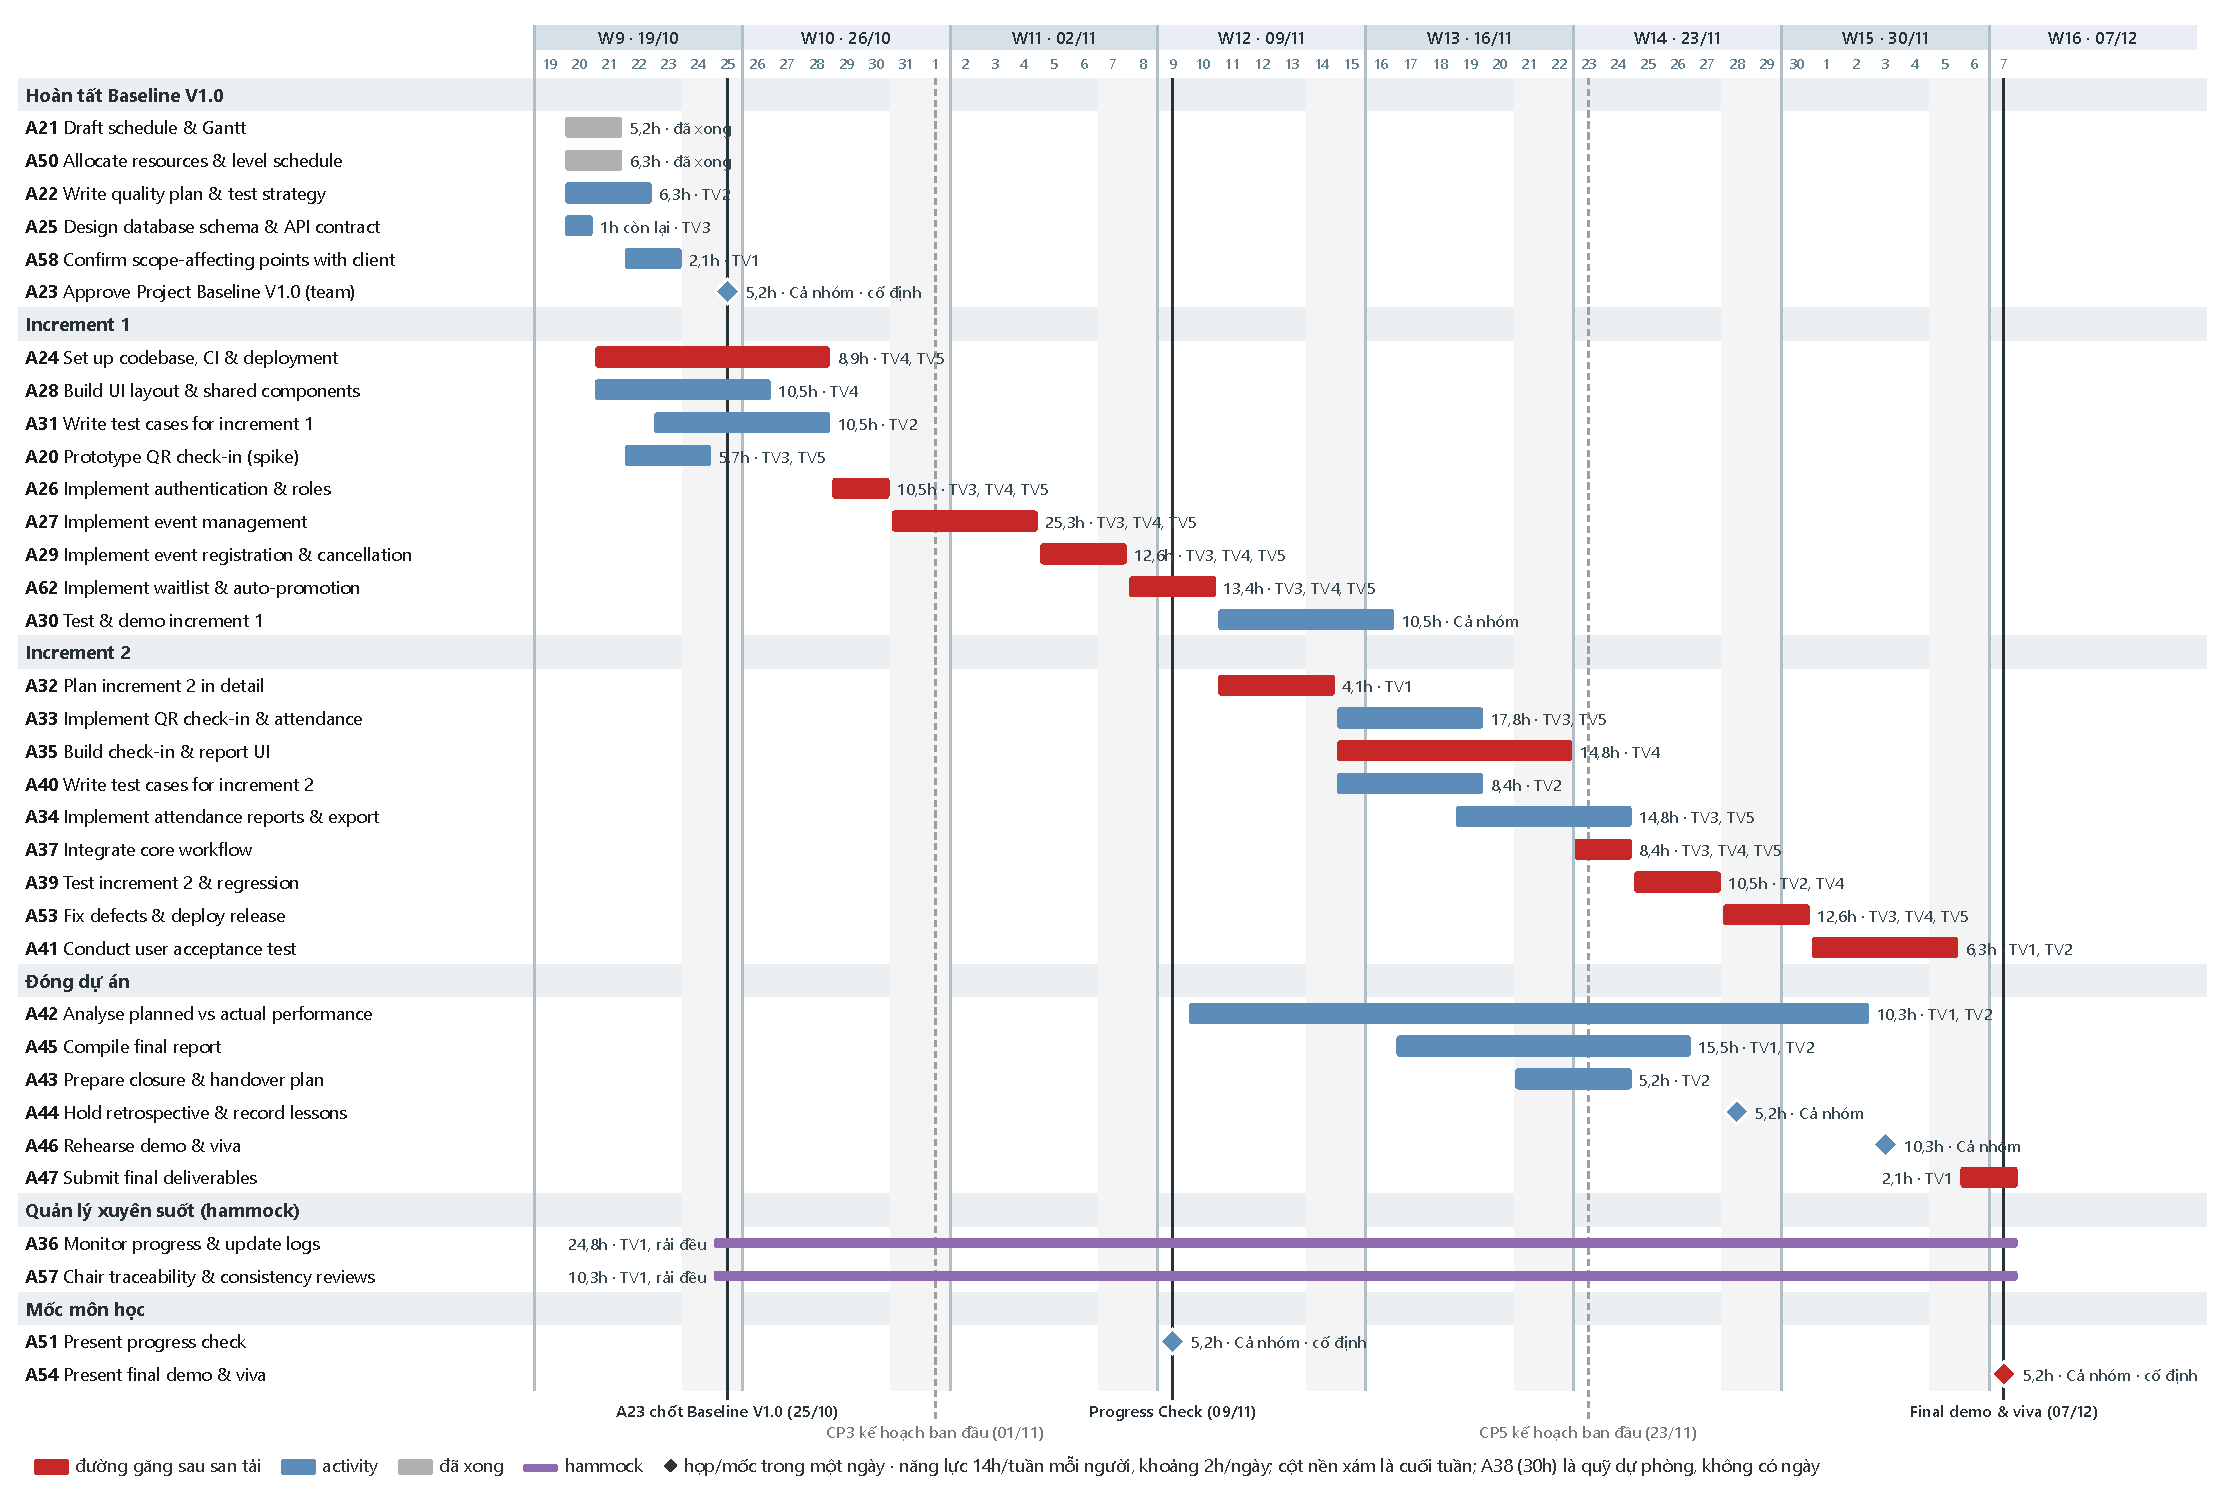
\includegraphics[width=\linewidth,height=0.88\textheight,keepaspectratio]{image/gantt.pdf}
\caption{Gantt Baseline V1.0 (đã san tải, 14 giờ/tuần mỗi người, A23 họp 25/10); thanh đỏ là đường găng}
\label{fig:gantt}
\end{figure}
\end{landscape}

\textbf{Cost baseline.} Đơn vị là giờ người, không quy đổi VND (E04). Các activity làm trước khi ước lượng (A01--A15, A49, A55, A59, A61) không có số ước lượng, chỉ ghi giờ thực tế ở tab Time Tracking (đang thu theo I02).

\begingroup\tblsetup\tblzebra
\begin{longtable}{L{4.6cm}L{7.4cm}>{\raggedleft\arraybackslash}p{2.2cm}}
\caption{Cost baseline theo giai đoạn (giờ người)}\label{tab:cost-baseline}\\
\toprule
\rowcolor{tblheadbg}\textbf{Giai đoạn} & \textbf{Activity} & \textbf{Effort} \\
\midrule
\endfirsthead
\toprule
\rowcolor{tblheadbg}\textbf{Giai đoạn} & \textbf{Activity} & \textbf{Effort} \\
\midrule
\endhead
\bottomrule
\endlastfoot
Lập kế hoạch Task 2 & A16, A17, A18, A19, A22, A25, A21, A20, A50, A58, A23 & 70,2 \\
Increment 1 & A24, A26, A28, A31, A27, A29, A62, A30 & 102,2 \\
Increment 2 và kiểm thử & A32, A33, A34, A35, A40, A37, A51, A39, A53, A41 & 102,9 \\
Đóng dự án & A42, A43, A44, A45, A46, A47, A54 & 53,8 \\
Quản lý xuyên suốt & A36, A57 & 35,1 \\
\textbf{Cộng effort kế hoạch} &  & \textbf{364,2} \\
Quỹ dự phòng A38 (change event, tách riêng) & A38 & 30,0 \\
\textbf{Cost baseline} &  & \textbf{394,2} \\
\end{longtable}
\endgroup

Quỹ A38 nằm trong giờ dư của TV2--TV5 (mục~\ref{sec:2-10}), nhưng lịch không còn ngày dự trữ: nếu change event rơi vào chuỗi găng thì nhóm cắt Could rồi Should hoặc lập Baseline V2.0. Rủi ro trễ lịch được theo dõi ở R15 (TV1 cập nhật R15 và Risk History ngày 21/10).

\kiemtra{Lịch, Gantt và cost baseline do AI hỗ trợ tính ngày 20/10, chạy lại 21/10 khi TV1 chốt A23 ngày 25/10 (\texttt{tools/schedule/baseline-v1-a23-25-10.json}); TV1 chọn phương án, nhóm xác nhận tại A23 ngày 25/10 (chọn V0). Bản chi tiết: \texttt{docs/task2/2.11-schedule.md}.}

\section{Baseline V1.0}
\label{sec:2-12}
Baseline V1.0 là mốc nội bộ của nhóm (CP2), không phải milestone của môn học (Q16); client không duyệt toàn bộ baseline (P05). Nội dung gồm:
\begin{itemize}
  \item \textbf{Phạm vi:} toàn bộ yêu cầu Must (mục~\ref{sec:1-4}); Should và Could chỉ làm khi còn thời gian, cắt theo thứ tự Could rồi Should, không bỏ core workflow.
  \item \textbf{Sản phẩm và activity:} PBS, PD-01 đến PD-05, PFD và mạng activity (mục~\ref{sec:2-1}--\ref{sec:2-4}, gồm L1--L11).
  \item \textbf{Ước lượng và chi phí:} 364,2 giờ người effort kế hoạch, cộng quỹ dự phòng A38 30 giờ, cost baseline 394,2 giờ người (mục~\ref{sec:2-6}, Bảng~\ref{tab:cost-baseline}).
  \item \textbf{Lịch:} Bảng~\ref{tab:schedule} và Hình~\ref{fig:gantt}; CP3 11--16/11, Progress Check 09/11, UAT 01--05/12, demo 07/12, không còn ngày dự trữ.
  \item \textbf{Tài nguyên:} 14 giờ/tuần mỗi người, phân vai và tải theo tuần ở mục~\ref{sec:2-10}.
  \item \textbf{Rủi ro:} sổ rủi ro cấp activity và activity phản hồi rủi ro (mục~\ref{sec:2-8}, \ref{sec:2-9}); rủi ro lịch chính là R15.
\end{itemize}

Nhóm xác nhận cả 18 mục của checklist A23 tại họp 15h Chủ nhật 25/10/2026 (TV1 báo ngày 27/10), trong đó chọn phương án chia giờ V0 (giữ lịch, không còn ngày dự trữ trước demo 07/12) và giữ GitLab, Jenkins do TV3 giữ. Khoảng đệm bằng không là rủi ro lịch nhóm chấp nhận; nếu A27 trễ quá một ngày thì TV1 xem xét cắt REQ-21 (Should).

\kiemtra{Biên bản chi tiết ở tab Biên bản CP (dòng CP2 bổ sung). Chưa xuất \texttt{v1.0.pdf} và chưa gắn tag \texttt{baseline-v1.0}; khi xong thì đưa bản đầy đủ vào Phụ lục~\ref{app:baselines} và ghi ngày tag.}
